%%%%%%%%%%%%%%%%%%%%%%% file template.tex %%%%%%%%%%%%%%%%%%%%%%%%%
%
% This is a general template file for the LaTeX package SVJour3
% for Springer journals.          Springer Heidelberg 2010/09/16
%
% Copy it to a new file with a new name and use it as the basis
% for your article. Delete % signs as needed.
%
% This template includes a few options for different layouts and
% content for various journals. Please consult a previous issue of
% your journal as needed.
%
%%%%%%%%%%%%%%%%%%%%%%%%%%%%%%%%%%%%%%%%%%%%%%%%%%%%%%%%%%%%%%%%%%%
%
% First comes an example EPS file -- just ignore it and
% proceed on the \documentclass line
% your LaTeX will extract the file if required
\begin{filecontents*}{example.eps}
%!PS-Adobe-3.0 EPSF-3.0
%%BoundingBox: 19 19 221 221
%%CreationDate: Mon Sep 29 1997
%%Creator: programmed by hand (JK)
%%EndComments
gsave
newpath
  20 20 moveto
  20 220 lineto
  220 220 lineto
  220 20 lineto
closepath
2 setlinewidth
gsave
  .4 setgray fill
grestore
stroke
grestore
\end{filecontents*}
%
\RequirePackage{fix-cm}
%
%\documentclass{svjour3}                     % onecolumn (standard format)
%\documentclass[smallcondensed]{svjour3}     % onecolumn (ditto)
\documentclass[smallextended]{svjour3}       % onecolumn (second format)
%\documentclass[twocolumn]{svjour3}          % twocolumn
%
\smartqed  % flush right qed marks, e.g. at end of proof
%
\usepackage{graphicx}
\usepackage{textcomp}
\usepackage[super]{nth}
\usepackage{subfigure}
\usepackage{booktabs}
\usepackage{multirow}


%
% \usepackage{mathptmx}      % use Times fonts if available on your TeX system
%
% insert here the call for the packages your document requires
%\usepackage{latexsym}
% etc.
%
% please place your own definitions here and don't use \def but
% \newcommand{}{}
%
% Insert the name of "your journal" with
% \journalname{myjournal}
%
\begin{document}

\title{On Usage of Non-Volatile Memory as Primary Storage for Database Management Systems
\thanks{The research leading to these results has received funding from the European Union\textquotesingle s 7th Framework Programme under grant agreement number 318633, the Ministry of Science and Technology of Spain under contract TIN2015-65316-P, and a HiPEAC collaboration grant awarded to Naveed Ul Mustafa.
%Grants or other notes
%about the article that should go on the front page should be
%placed here. General acknowledgments should be placed at the end of the article.
}
}
%\subtitle{Do you have a subtitle?\\ If so, write it here}

\titlerunning{Naveed Ul MUSTAFA et al. On Usage of NVM as Primary Storage for DBMS}        % if too long for running head

\author{Naveed Ul Mustafa \and Adri\`{a} Armejach  \and
        Ozcan Ozturk \and  Adri\'{a}n Cristal 
        \and \\ Osman S. Unsal
         %etc.
}

%\authorrunning{Short form of author list} % if too long for running head

\institute{N. Ul Mustafa \at
              Department of Computer Engineering, Bilkent University, Ankara, Turkey. \\
              Present Address: Department of Computer Engineering, TED University, Ankara, Turkey.\\
              %Tel.: +123-45-678910\\
              %Fax: +123-45-678910\\
              \email{naveed.ul.mustafa0083@gmail.com}           %  \\
%             \emph{Present address:} of F. Author  %  if needed
           \and
           A. Armejach \at
              Barcelona Supercomputing Center (BSC), Barcelona, Spain and Universitat Polit\`{e}cnica de Catalunya (UPC), Barcelona, Spain.
           \and O. Ozturk \at
              Department of Computer Engineering, Bilkent University, Ankara 06800, Turkey.
           \and A. Cristal \at 
              Barcelona Supercomputing Center (BSC), Barcelona, Spain.
           \and O. S. Unsal \at
              Barcelona Supercomputing Center (BSC), Barcelona, Spain.
}

\date{Received: date / Accepted: date}
% The correct dates will be entered by the editor


\maketitle

\begin{abstract}
\begin{abstract}  
Test time scaling is currently one of the most active research areas that shows promise after training time scaling has reached its limits.
Deep-thinking (DT) models are a class of recurrent models that can perform easy-to-hard generalization by assigning more compute to harder test samples.
However, due to their inability to determine the complexity of a test sample, DT models have to use a large amount of computation for both easy and hard test samples.
Excessive test time computation is wasteful and can cause the ``overthinking'' problem where more test time computation leads to worse results.
In this paper, we introduce a test time training method for determining the optimal amount of computation needed for each sample during test time.
We also propose Conv-LiGRU, a novel recurrent architecture for efficient and robust visual reasoning. 
Extensive experiments demonstrate that Conv-LiGRU is more stable than DT, effectively mitigates the ``overthinking'' phenomenon, and achieves superior accuracy.
\end{abstract}  
%Insert your abstract here. Include keywords, PACS and mathematical subject classification numbers as needed. 
\keywords{Non volatile memory \and Relational DBMS \and Storage engine}
% \PACS{PACS code1 \and PACS code2 \and more}
% \subclass{MSC code1 \and MSC code2 \and more}
\end{abstract}

\section{Introduction}
\label{sec:introduction}
The business processes of organizations are experiencing ever-increasing complexity due to the large amount of data, high number of users, and high-tech devices involved \cite{martin2021pmopportunitieschallenges, beerepoot2023biggestbpmproblems}. This complexity may cause business processes to deviate from normal control flow due to unforeseen and disruptive anomalies \cite{adams2023proceddsriftdetection}. These control-flow anomalies manifest as unknown, skipped, and wrongly-ordered activities in the traces of event logs monitored from the execution of business processes \cite{ko2023adsystematicreview}. For the sake of clarity, let us consider an illustrative example of such anomalies. Figure \ref{FP_ANOMALIES} shows a so-called event log footprint, which captures the control flow relations of four activities of a hypothetical event log. In particular, this footprint captures the control-flow relations between activities \texttt{a}, \texttt{b}, \texttt{c} and \texttt{d}. These are the causal ($\rightarrow$) relation, concurrent ($\parallel$) relation, and other ($\#$) relations such as exclusivity or non-local dependency \cite{aalst2022pmhandbook}. In addition, on the right are six traces, of which five exhibit skipped, wrongly-ordered and unknown control-flow anomalies. For example, $\langle$\texttt{a b d}$\rangle$ has a skipped activity, which is \texttt{c}. Because of this skipped activity, the control-flow relation \texttt{b}$\,\#\,$\texttt{d} is violated, since \texttt{d} directly follows \texttt{b} in the anomalous trace.
\begin{figure}[!t]
\centering
\includegraphics[width=0.9\columnwidth]{images/FP_ANOMALIES.png}
\caption{An example event log footprint with six traces, of which five exhibit control-flow anomalies.}
\label{FP_ANOMALIES}
\end{figure}

\subsection{Control-flow anomaly detection}
Control-flow anomaly detection techniques aim to characterize the normal control flow from event logs and verify whether these deviations occur in new event logs \cite{ko2023adsystematicreview}. To develop control-flow anomaly detection techniques, \revision{process mining} has seen widespread adoption owing to process discovery and \revision{conformance checking}. On the one hand, process discovery is a set of algorithms that encode control-flow relations as a set of model elements and constraints according to a given modeling formalism \cite{aalst2022pmhandbook}; hereafter, we refer to the Petri net, a widespread modeling formalism. On the other hand, \revision{conformance checking} is an explainable set of algorithms that allows linking any deviations with the reference Petri net and providing the fitness measure, namely a measure of how much the Petri net fits the new event log \cite{aalst2022pmhandbook}. Many control-flow anomaly detection techniques based on \revision{conformance checking} (hereafter, \revision{conformance checking}-based techniques) use the fitness measure to determine whether an event log is anomalous \cite{bezerra2009pmad, bezerra2013adlogspais, myers2018icsadpm, pecchia2020applicationfailuresanalysispm}. 

The scientific literature also includes many \revision{conformance checking}-independent techniques for control-flow anomaly detection that combine specific types of trace encodings with machine/deep learning \cite{ko2023adsystematicreview, tavares2023pmtraceencoding}. Whereas these techniques are very effective, their explainability is challenging due to both the type of trace encoding employed and the machine/deep learning model used \cite{rawal2022trustworthyaiadvances,li2023explainablead}. Hence, in the following, we focus on the shortcomings of \revision{conformance checking}-based techniques to investigate whether it is possible to support the development of competitive control-flow anomaly detection techniques while maintaining the explainable nature of \revision{conformance checking}.
\begin{figure}[!t]
\centering
\includegraphics[width=\columnwidth]{images/HIGH_LEVEL_VIEW.png}
\caption{A high-level view of the proposed framework for combining \revision{process mining}-based feature extraction with dimensionality reduction for control-flow anomaly detection.}
\label{HIGH_LEVEL_VIEW}
\end{figure}

\subsection{Shortcomings of \revision{conformance checking}-based techniques}
Unfortunately, the detection effectiveness of \revision{conformance checking}-based techniques is affected by noisy data and low-quality Petri nets, which may be due to human errors in the modeling process or representational bias of process discovery algorithms \cite{bezerra2013adlogspais, pecchia2020applicationfailuresanalysispm, aalst2016pm}. Specifically, on the one hand, noisy data may introduce infrequent and deceptive control-flow relations that may result in inconsistent fitness measures, whereas, on the other hand, checking event logs against a low-quality Petri net could lead to an unreliable distribution of fitness measures. Nonetheless, such Petri nets can still be used as references to obtain insightful information for \revision{process mining}-based feature extraction, supporting the development of competitive and explainable \revision{conformance checking}-based techniques for control-flow anomaly detection despite the problems above. For example, a few works outline that token-based \revision{conformance checking} can be used for \revision{process mining}-based feature extraction to build tabular data and develop effective \revision{conformance checking}-based techniques for control-flow anomaly detection \cite{singh2022lapmsh, debenedictis2023dtadiiot}. However, to the best of our knowledge, the scientific literature lacks a structured proposal for \revision{process mining}-based feature extraction using the state-of-the-art \revision{conformance checking} variant, namely alignment-based \revision{conformance checking}.

\subsection{Contributions}
We propose a novel \revision{process mining}-based feature extraction approach with alignment-based \revision{conformance checking}. This variant aligns the deviating control flow with a reference Petri net; the resulting alignment can be inspected to extract additional statistics such as the number of times a given activity caused mismatches \cite{aalst2022pmhandbook}. We integrate this approach into a flexible and explainable framework for developing techniques for control-flow anomaly detection. The framework combines \revision{process mining}-based feature extraction and dimensionality reduction to handle high-dimensional feature sets, achieve detection effectiveness, and support explainability. Notably, in addition to our proposed \revision{process mining}-based feature extraction approach, the framework allows employing other approaches, enabling a fair comparison of multiple \revision{conformance checking}-based and \revision{conformance checking}-independent techniques for control-flow anomaly detection. Figure \ref{HIGH_LEVEL_VIEW} shows a high-level view of the framework. Business processes are monitored, and event logs obtained from the database of information systems. Subsequently, \revision{process mining}-based feature extraction is applied to these event logs and tabular data input to dimensionality reduction to identify control-flow anomalies. We apply several \revision{conformance checking}-based and \revision{conformance checking}-independent framework techniques to publicly available datasets, simulated data of a case study from railways, and real-world data of a case study from healthcare. We show that the framework techniques implementing our approach outperform the baseline \revision{conformance checking}-based techniques while maintaining the explainable nature of \revision{conformance checking}.

In summary, the contributions of this paper are as follows.
\begin{itemize}
    \item{
        A novel \revision{process mining}-based feature extraction approach to support the development of competitive and explainable \revision{conformance checking}-based techniques for control-flow anomaly detection.
    }
    \item{
        A flexible and explainable framework for developing techniques for control-flow anomaly detection using \revision{process mining}-based feature extraction and dimensionality reduction.
    }
    \item{
        Application to synthetic and real-world datasets of several \revision{conformance checking}-based and \revision{conformance checking}-independent framework techniques, evaluating their detection effectiveness and explainability.
    }
\end{itemize}

The rest of the paper is organized as follows.
\begin{itemize}
    \item Section \ref{sec:related_work} reviews the existing techniques for control-flow anomaly detection, categorizing them into \revision{conformance checking}-based and \revision{conformance checking}-independent techniques.
    \item Section \ref{sec:abccfe} provides the preliminaries of \revision{process mining} to establish the notation used throughout the paper, and delves into the details of the proposed \revision{process mining}-based feature extraction approach with alignment-based \revision{conformance checking}.
    \item Section \ref{sec:framework} describes the framework for developing \revision{conformance checking}-based and \revision{conformance checking}-independent techniques for control-flow anomaly detection that combine \revision{process mining}-based feature extraction and dimensionality reduction.
    \item Section \ref{sec:evaluation} presents the experiments conducted with multiple framework and baseline techniques using data from publicly available datasets and case studies.
    \item Section \ref{sec:conclusions} draws the conclusions and presents future work.
\end{itemize}
\section{Background}
\label{sec:background}
\noindent In this section, we first describe in detail the properties of NVM technologies, highlighting the implications these might have in the design of a DBMS. We then describe currently available NVM hardware and  system software to manage NVM.


\subsection{Characteristics of NVM}
\noindent \textbf{Data access latency:} Read latencies for NVM technologies will certainly be significantly lower than those of conventional disks. However, since NVM devices are still under development, sources quote varying read latencies. For example, the read latency for STT-RAM ranges from 1 to 20ns, and PC-RAM is expected to be around 50ns ~\cite{arulraj2015let,wang2013low,perez2010non}. Nonetheless, read latency of some NVM technologies is expected to be similar to that of DRAM ~\cite{mittal2016survey,arulraj2015let,wang2013low,chang2012limits,arulraj2016write,oukid2014sofort,chatzistergiou2015rewind}, which is typically around 60ns.

PC-RAM and R-RAM are reported to have a higher write latency compared to DRAM, but STT-RAM also outperforms DRAM in this regard ~\cite{arulraj2015let,wang2013low}. However, the write latency is typically not in the critical path, since it can be tolerated by using buffers ~\cite{qureshi2009scalable}.

\noindent\textbf{Density:} NVM technologies provide higher densities than DRAM, which makes them a good candidate to be used as main memory as well as primary storage, particularly in embedded systems~\cite{huang2012register}. For example, PC-RAM provides 2 to 4 times higher density as compared to DRAM~\cite{qureshi2009scalable}. Future NVMs are expected to have higher capacity and better scalability than DRAM \cite{oukid2015instant,chakrabarti2014atlas,zhang2015study,viglas2014write}
, and it is expected to scale to lower technology nodes as opposed to DRAM.

\noindent\textbf{Endurance:} The maximum number of writes a memory cell can withstand is lower for most NVM 
technologies when compared to DRAM ~\cite{qureshi2009scalable,zhou2009durable}. Specifically, PC-RAM, R-RAM, 
and STT-RAM have projected endurances of $10^{10}$, $10^{8}$, and $10^{15}$ respectively;  as compared to 
$10^{16}$ for DRAM ~\cite{arulraj2015let}. On the other hand, NVMs exhibit higher endurance than flash 
memory technologies ~\cite{wang2013low}.

\noindent\textbf{Energy consumption:} Since NVM does not need a refresh cycle to maintain data states in memory cells like a  DRAM, 
they are more energy efficient. A main memory designed using PC-RAM technology consumes significantly lower per access write energy as compared to DRAM~\cite{zhou2009durable}. Other NVM technologies also have similar lower energy consumption per bit when compared to DRAM~\cite{arulraj2015let,perez2010non}.

In addition to the features listed above, NVM technologies also provide byte-addressability like DRAM and persistency like disks. Due to these features, NVMs are starting to appear in embedded and energy-critical devices and are expected to play a major role in future computing systems. Companies like Intel and Micron have launched the 3D XPoint memory technology, which features non-volatility \cite{3DXPoint}. Intel has also introduced new instructions to support the usage of persistent memory at the instruction set architecture (ISA) level~\cite{intel2016architecture}.

\subsection{Available NVM hardware}\label{NVDIMM}

While NVM hardware has been available in recent years, it has mainly been used to implement Solid State Disks (SSD) using the NVM Express (NVMe) interface. This technology is not suitable as a DRAM replacement due to its endurance and latency properties. Researchers have been anticipating the arrival of Dual Inline Memory Modules (DIMM) based on NVM to substitute traditional DRAM DIMMs for a long time. Recently, in April 2019, Intel has released its 3D Xpoint DIMM based on NVM technology~\cite{hirofuchi2019preliminary}.

As shown in Fig.~\ref{3DXPointInterface}, 3D Xpoint DIMMs connect to the memory bus and communicate with a processor through the integrated memory controller (iMC). Each iMC can connect to up to three DIMMs~\cite{peng2019system,yang2019empirical}. A non-standard protocol, DDR-T, is followed for communication between processors and 3D XPoint DIMM. Intel\textquotesingle s Cascade Lake processors are yet the only ones to support 3D Xpoint memory.  As each processor supports two iMCs, six DIMMs are supported in total~\cite{peng2019system,yang2019empirical,izraelevitz2019basic}.

3D XPoint DIMMs can operate in two different modes: Memory and App Direct. Memory mode uses NVM to expand main memory without providing the feature of persistency, while regular DRAM serves as a cache for NVM. In this mode, operating system and CPU see the NVM memory as a volatile extension of main memory. In App Direct mode, NVM is used as a separate persistent memory and does not use DRAM as cache. App Direct mode provides an application direct access to data residing in NVM without interference of the operating system and with byte-addressability. However, it requires an NVM-aware file system to allocate, name, and access persistent data.

\begin{figure}
\centering
\includegraphics[width=.5\textwidth]{3DXPointInterface.eps}
\caption{Overview of 3D XPoint Memory\textquotesingle s interface with CPU}
\label{3DXPointInterface}
\end{figure}

\subsection{System software for NVM}

Using NVM as primary storage necessitates modifications not only in application software but also in system software in order to 
take advantage of NVM features. A traditional file system (FS) accesses the storage through a block layer. If a disk is replaced by NVM without any modifications in
the FS, the NVM storage will still be accessed at block level granularity. Hence, we will not be able to take advantage of the byte-addressability feature of NVM. 

For this reason, researchers have developed purpose-built file systems such as NOn Volatile memory Accelerated (NOVA) \cite{xu2016nova} and persistent memory file System (PMFS) ~\cite{dulloor2014system,githubPMFS}. Both file systems expose NVM to an application by providing direct access through a memory map (mmap) interface. As this work uses PMFS, we discuss it in more detail below.

PMFS is an open-source POSIX compliant FS developed by Intel Research. It offers two key features in order to facilitate usage of NVM.  
First, PMFS does not maintain a separate address space for NVM. In other words, both main memory and NVM use the same address space. This implies that there is no need to copy data from NVM to DRAM to make it accessible to an application. A process can directly access file system protected data stored in NVM at byte level granularity.

Second, in a traditional FS stored blocks can be accessed in two ways: (i) file I/O and (ii) memory mapped I/O. PMFS implements file I/O in a similar way to a traditional FS. However, the implementation of memory mapped I/O differs. In a traditional FS, memory mapped I/O would first copy pages to DRAM~\cite{dulloor2014system} from where an application can examine those pages. PMFS avoids this copy overhead by mapping NVM pages directly into the address space of a process. Fig.~\ref{Fig1} from~\cite{dulloor2014system} compares a traditional FS with PMFS.

%\subsection{NVM DIMM}
%Dual In-line Memory Module using NVM have been long anticipated by communit of memory reserachers. Recently, Intel has annnounced and made commercially available its product named Intel's 3D XPoint memory as an NVM DIMM.

\begin{figure}
\centering
\includegraphics[width=100mm]{Fig1.eps}
\caption{Comparison of traditional FS and PMFS. ``mmap'' refers to the system call for memory mapped I/O operation. 
``mmu'' is the memory management unit responsible for address mappings}
\label{Fig1}
\end{figure}




%\section{Design Choices}
\label{sec:Implications}
\noindent In this section, we discuss the possible memory hierarchy designs when including NVM in a system. We also discuss the high-level modifications necessary in a traditional disk-optimized DBMS in order to take full advantage of NVM hardware.
\subsection{Memory Hierarchy Designs for an NVM-Based DBMS}

With features of byte-addressability, low latency and high capacity, NVM has the potential to replace traditional disks as well as main memory \cite{chang2012limits}. Fig.~\ref{Fig2} shows different options that might be considered when including NVM into the system. Fig.~\ref{Fig2a} depicts a traditional approach, where the intermediate state - including logs, data buffers, and partial query state - is stored in DRAM to hide disk latencies for data that is currently in use; while the bulk of the relational data is stored in a  disk.

Given the favorable characteristics of NVM over the other technologies, an option might be to replace both DRAM and disk storage 
using NVM (Fig.~\ref{Fig2b}). However, such a drastic change would require a complete redesign of current operating systems and 
application software. In addition, NVM technology is still not mature enough in terms of endurance to be used as a DRAM replacement. 
Hence, we advocate for a platform that still has a layer of DRAM memory, like \cite{kimura2015foedus}, where the disk is completely or partially replaced using NVM, 
as shown in Fig.~\ref{Fig2c} (NVM-Disk).

Using this approach, we can retain the programmability of current systems by still having a layer of DRAM, thereby exploiting DRAM's fast read and write access latencies for temporary data structures and application code. In addition, it allows the possibility to directly access the bulk of the database relational data by using a file system such as PMFS, taking full advantage of NVM technology, which allows the system to leverage NVM's byte-addressability and to avoid API overheads~\cite{huang2014nvram} present in current FSs. Unlike an in-memory DBMS, such a setup does not need large pools of DRAM since temporary data is orders of magnitude smaller than the actual relational database stored in NVM. We believe this is a realistic scenario for future systems integrating NVM, with room for small variations such as NVM alongside DRAM to store persistent temporary data structures, or having traditional disks to store cold data.

\begin{figure} %[!htbp]
\centering     %%% not \center
\subfigure[Traditional design]{\label{Fig2a}\includegraphics[width=27mm]{Fig2a.eps}}
\subfigure[All-in-NVM]{\label{Fig2b}\includegraphics[width=27mm]{Fig2b.eps}}
\subfigure[NVM-Disk]{\label{Fig2c}\includegraphics[width=27mm]{Fig2c.eps}}
\caption{NVM placement in the memory hierarchy of a computing system}
\label{Fig2}
\end{figure}

\subsection{Potential Modifications in a Traditional DBMS}~\label{modList}
Using a traditional disk-based database with NVM storage will not take full advantage of NVM's features. Some important components of the DBMS need to be modified or removed when using NVM as a primary storage. 

\noindent\textbf{Avoid the block level access:} Traditional design of a DBMS uses a disk as a primary storage. Since disks favor sequential accesses, database systems hide disk latencies by issuing fewer but larger disk accesses in the form of a data block~\cite{schindler2002track}. 

Unfortunately, block level I/O causes extra data movement. For example, if a transaction updates a single byte of a tuple, it still needs to write the whole block of data to the disk. On the other hand, block level access provides good data locality.
 
Since NVM is byte-addressable, we can read and write only the required byte(s). However, reducing the data retrieval granularity down to a byte level eliminates the advantage of data locality altogether. A good compromise is to reduce the block size in such a way that the overhead of the block I/O is reduced to an acceptable level, while at the same time the application benefits from some degree of data locality. 
 
\noindent\textbf{Remove internal buffer cache of DBMS:} DBMSs usually maintain an internal buffer cache. Whenever a tuple is to be accessed, first its disk address has to be calculated. If the corresponding block of data is not found in the internal buffer cache, then it is read from disk and stored in the internal buffer cache \cite{debrabant2013anti}. 
 
This approach is unnecessary in an NVM-based database design. If the NVM address space is made visible to a process, then there is no need to copy data blocks. It is more efficient to refer to the tuple directly by its address. However, we need an NVM-aware FS, such as PMFS, to enable direct access to the NVM address space by a process.
 



\subsection{Discussion}
NVM provides the promising features of persistency, like disk storage; and byte-addressability, like DRAM. However, NVMs
have certain limitations such as lower endurance compared to DRAM \cite{arulraj2015let} and a disparity between the read and write latencies \cite{pelley2014memory}. 
Furthermore, different NVM technologies differ from each other in term of these features \cite{arulraj2015let}.

 
A storage engine aiming to improve decision support
system (DSS) queries can be designed by taking advantage
of the common features of persistency and byte-addressability.
Since DSS queries are read dominant and perform a relatively
negligible number of write operations, the design should
not be influenced or sensitive to different endurance and write
latencies found across NVM technologies. Furthermore, NVM technologies
are projected to provide read latencies similar to DRAM \cite{mittal2016survey,arulraj2015let,wang2013low,chang2012limits}.
Therefore, reading data directly from NVM storage should be comparable in terms
of access latency to reading application data stored in DRAM.

 
Usage of NVM as primary storage can also impact
other components of a DBMS besides those mentioned
in Section \ref{modList}. For example, if internal buffers are not
employed and all updates are materialized directly into the
NVM address space then the need and criticality of the redo
log can be relaxed \cite{huang2014nvram}. However, the undo log will still be
needed to recover from a system failure. These important aspects are
out of the scope of this work and we will focus on storage engine modifications.

\begin{figure*}  [!htbp]
\centering     %%% not \center
\subfigure[PostgreSQL storage engine]{\label{Fig3a}\includegraphics[width=38mm]{Fig4.eps}}
\subfigure[Modified storage engine - SE1]{\label{Fig3b}\includegraphics[width=38mm]{Fig5New.eps}}
\subfigure[Modified storage engine - SE2]{\label{Fig3c}\includegraphics[width=38mm]{Fig6New.eps}}
\caption{High level view of read and write memory operations in PostgreSQL (read as ``pg'' in short form) and modified SEs}
\label{Fig3}
\end{figure*}
 

\section{Design Choices}
\label{sec:Implications}
\noindent In this section, we discuss the possible memory hierarchy designs when including NVM in a system. We also discuss the high-level modifications necessary in a traditional disk-optimized DBMS in order to take full advantage of NVM hardware.
\subsection{Memory Hierarchy Designs for an NVM-Based DBMS}

With features of byte-addressability, low latency and high capacity, NVM has the potential to replace traditional disks as well as main memory \cite{chang2012limits}. Fig.~\ref{Fig2} shows different options that might be considered when including NVM into the system. Fig.~\ref{Fig2a} depicts a traditional approach, where the intermediate state - including logs, data buffers, and partial query state - is stored in DRAM to hide disk latencies for data that is currently in use; while the bulk of the relational data is stored in a  disk.

Given the favorable characteristics of NVM over the other technologies, an option might be to replace both DRAM and disk storage 
using NVM (Fig.~\ref{Fig2b}). However, such a drastic change would require a complete redesign of current operating systems and 
application software. In addition, NVM technology is still not mature enough in terms of endurance to be used as a DRAM replacement. 
Hence, we advocate for a platform that still has a layer of DRAM memory, like \cite{kimura2015foedus}, where the disk is completely or partially replaced using NVM, 
as shown in Fig.~\ref{Fig2c} (NVM-Disk). 

Using this approach, we can retain the programmability of current systems by still having a layer of DRAM, thereby exploiting DRAM's fast read and write access latencies for temporary data structures and application code. In addition, it allows the possibility to directly access the bulk of the database relational data by using a file system such as PMFS, taking full advantage of NVM technology, which allows the system to leverage NVM's byte-addressability and to avoid API overheads~\cite{huang2014nvram} present in current FSs. Unlike an in-memory DBMS, such a setup does not need large pools of DRAM since temporary data is orders of magnitude smaller than the actual relational database stored in NVM. We believe this is a realistic scenario for future systems integrating NVM, with room for small variations such as NVM alongside DRAM to store persistent temporary data structures, or having traditional disks to store cold data.

As explained in Section~\ref{NVDIMM}, 3D XPoint memory can operate in two different modes. Memory mode is similar to a traditional design (Fig.~\ref{Fig2a}), as the 3D XPoint DIMMS are not considered as persistent memory but as the actual DRAM address space. In this mode the DRAM DIMMs are transparently used as a cache for the 3D XPoint DIMMs. This does not change the system view from an application's point of view, and makes sense if one wants to use 3D XPoint DIMMs as if they were large-capacity DRAM DIMMs. However, the App Direct mode would fit into the NVM-Disk (Fig.~\ref{Fig2c}) category. Applications still see DRAM DIMMs as a layer of volatile memory, but can also directly access the 3D XPoint DIMMs via mmap interfaces that enable byte-addressability. The system we consider and later evaluate would be based on a setup similar to that offered by 3D XPoint\textquotesingle s  App Direct mode.


%\textcolor{blue}{Memory mode operation of 3D XPoint memory (explained in Section \ref{NVDIMM}) uses a configuration similar to  NVM-Disk (see Fig.~\ref{Fig2c}) with some differences. Although DRAM is used as a cache in memory mode, 3D Xpoint memory acts as volatile extension of DRAM and sits between storage and DRAM in the memory hierarchy. Fig.~\ref{MemOverview3DXPoint}, based on \cite{peng2019system}, shows the logical view of memory hierarchy in App Direct and Memory mode operation of 3D XPoint memory.}

\begin{figure} %[!htbp]
\centering     %%% not \center
\subfigure[Traditional design]{\label{Fig2a}\includegraphics[width=27mm]{Fig2a.eps}}
\subfigure[All-in-NVM]{\label{Fig2b}\includegraphics[width=27mm]{Fig2b.eps}}
\subfigure[NVM-Disk]{\label{Fig2c}\includegraphics[width=27mm]{Fig2c.eps}}
\caption{NVM placement in the memory hierarchy of a computing system}
\label{Fig2}
\end{figure}

%\begin{figure} %[!htbp]
%\centering     %%% not \center
%\subfigure[Memory Mode]{\label{MemMode}\includegraphics[width=35mm]{3DXPointMmeoryModeConfig.eps}}
%\hspace{5pt}
%\subfigure[Direct Access Mode]{\label{DAXMode}\includegraphics[width=35mm]{3DXPointAppDirectModeConfig.eps}}
%\caption{Overview of memory hiearchy in Memory and Direct Access Mode of 3D XPoint Memory}
%\label{MemOverview3DXPoint}
%\end{figure}

\subsection{Potential Modifications in a Traditional DBMS}~\label{modList}
Using a traditional disk-based database with NVM storage will not take full advantage of NVM's features. Some important components of the DBMS need to be modified or removed when using NVM as a primary storage. 

\noindent\textbf{Avoid the block level access:} Traditional design of a DBMS uses a disk as a primary storage. Since disks favor sequential accesses, database systems hide disk latencies by issuing fewer but larger disk accesses in the form of a data block~\cite{schindler2002track}. 

Unfortunately, block level I/O causes extra data movement. For example, if a transaction updates a single byte of a tuple, it still needs to write the whole block of data to the disk. On the other hand, block level access provides good data locality.
 
Since NVM is byte-addressable, we can read and write only the required byte(s). However, reducing the data retrieval granularity down to a byte level eliminates the advantage of data locality altogether. A good compromise is to reduce the block size in such a way that the overhead of the block I/O is reduced to an acceptable level, while at the same time the application benefits from some degree of data locality. 
 
\noindent\textbf{Remove internal buffer cache of DBMS:} DBMSs usually maintain an internal buffer cache. Whenever a tuple is to be accessed, first its disk address has to be calculated. If the corresponding block of data is not found in the internal buffer cache, then it is read from disk and stored in the internal buffer cache \cite{debrabant2013anti}. 
 
This approach is unnecessary in an NVM-based database design. If the NVM address space is made visible to a process, then there is no need to copy data blocks. It is more efficient to refer to the tuple directly by its address. However, we need an NVM-aware FS, such as PMFS, to enable direct access to the NVM address space by a process.
 



\subsection{Discussion}
NVM provides the promising features of persistency, like disk storage; and byte-addressability, like DRAM. However, NVMs
have certain limitations such as lower endurance compared to DRAM \cite{arulraj2015let} and a disparity between the read and write latencies \cite{pelley2014memory}. 
Furthermore, different NVM technologies differ from each other in term of these features \cite{arulraj2015let}.

 
A storage engine aiming to improve decision support
system (DSS) queries can be designed by taking advantage
of the common features of persistency and byte-addressability.
Since DSS queries are read dominant and perform a relatively
negligible number of write operations, the design should
not be influenced or sensitive to different endurance and write
latencies found across NVM technologies. Furthermore, NVM technologies
are projected to provide read latencies similar to DRAM \cite{mittal2016survey,arulraj2015let,wang2013low,chang2012limits}.
Therefore, reading data directly from NVM storage should be comparable in terms
of access latency to reading application data stored in DRAM.

 
Usage of NVM as primary storage can also impact
other components of a DBMS besides those mentioned
in Section \ref{modList}. For example, if internal buffers are not
employed and all updates are materialized directly into the
NVM address space then the need and criticality of the redo
log can be relaxed \cite{huang2014nvram}. However, the undo log will still be
needed to recover from a system failure. These important aspects are
out of the scope of this work and we will focus on storage engine modifications.

\begin{figure*}  %[!htbp]
\centering     %%% not \center
\subfigure[PostgreSQL storage engine]{\label{Fig3a}\includegraphics[width=38mm]{Fig4.eps}}
\subfigure[Modified storage engine - SE1]{\label{Fig3b}\includegraphics[width=38mm]{Fig5New.eps}}
\subfigure[Modified storage engine - SE2]{\label{Fig3c}\includegraphics[width=38mm]{Fig6New.eps}}
\caption{High level view of read and write memory operations in PostgreSQL (read as ``pg'' in short form) and modified SEs}
\label{Fig3}
\end{figure*}
 

\section{A Case Study: P\MakeLowercase{ostgre}SQL}
\label{sec:CaseStudy}
\noindent PostgreSQL is an open source object-relational database system. It is fully atomicity, consistency, isolation, durability (ACID) 
compliant and runs on all major operating systems including Linux \cite{momjian2001postgresql}. In this section, we study the 
storage engine (SE) of PostgreSQL and apply necessary changes to make it NVM-aware. We first describe the read-write architecture 
of PostgreSQL and then explain our modifications.



\subsection{Read-Write Architecture of PostgreSQL}

Fig.~\ref{Fig3a} shows the original PostgreSQL architecture from the perspective of read and write file operations. 
The left column in the figure shows the operations performed by different software layers of PostgreSQL, while the right column 
shows the corresponding data movement activities. Note that in Fig.~\ref{Fig3a} we assume the disk has already been replaced 
by NVM hardware with PMFS as the file system. However, the same behavior would be expected using a regular disk and a traditional 
FS, since PostgreSQL heavily relies on file I/O for read and write operations and the file I/O APIs in PMFS are the same as those 
in a traditional FS.

The PostgreSQL server calls the services of the  \textit{Buffer Layer} which is responsible for maintaining an 
internal buffer cache. The buffer cache is used to keep a copy of the requested page which is read from the 
storage. Copies are kept in the cache as long as they are needed. If there is no free
slot available for a newly requested page then a replacement policy is used to select a victim. 
The victim is evicted from the buffer cache and if it is 
a dirty page, then it is also flushed back to the permanent storage.

Upon receiving a new request to read a page from storage, the \textit{Buffer Layer} finds a free buffer cache slot 
and gets a pointer to it. The free buffer slot and corresponding pointer are shown in Fig.~\ref{Fig3a} as \textit{Pg Buffer} and \textit{PgBufPtr}, respectively. The \textit{Buffer Layer} then passes the pointer to the \textit{File Layer}. Eventually, the \textit{File Layer} of PostgreSQL invokes the file read and write system calls implemented by the 
underlying FS. 

For a read operation, PMFS copies the data block from NVM to a kernel buffer and then the kernel copies the requested 
data block to an internal buffer slot pointed by \textit{PgBufPtr}. In the same way, two copies are made for write operation but in the opposite direction.

Hence, the SE of original PostgreSQL incurs two copy operations for each miss in the internal buffer cache. This is 
likely to become a big overhead for databases running queries on large datasets. However, since PMFS can map the entire NVM address space into the kernel's virtual address space~\cite{dulloor2014system}, the copy overhead can be avoided by making modifications in the SE. We apply these modifications in two incremental steps as described in 
the following subsections.

\subsection{SE1: Using Memory Mapped I/O}
In the first step towards leveraging the features of NVM, we replace the \textit{File Layer} of PostgreSQL by a 
new layer named \textit{MemMapped Layer}. As shown in Fig. \ref{Fig3b}, this layer still receives a pointer 
to a free buffer slot from the \textit{Buffer Layer}, but instead of using the file I/O interface, it uses the memory 
mapped I/O interface of PMFS. We term this storage engine \textit{SE1}.

\noindent\textbf{Read Operation:} When accessing a file for a read operation, we first open the file using the \verb+open()+ 
system call, same as in original PostgreSQL. Additionally, we create a mapping of the file using \verb+mmap()+. 
Since we are using PMFS, \verb+mmap()+ returns a pointer to the mapping of the file stored in NVM. The implementation of \verb+mmap()+ by PMFS provides the application with direct access to mapped pages of files residing in NVM.

As a result, we do not need to make an intermediate copy of the requested page from NVM into kernel buffers. We can 
directly copy the requested page into internal buffers of PostgreSQL by using an implicit \verb+memcpy()+ as shown in Fig. \ref{Fig3b}. When all requested operations on a given file are completed and it is not needed anymore, 
the file can be closed. Upon closing a file, we delete the mapping of the file by calling the \verb+munmap()+ function. 

\noindent\textbf{Write Operation:} The same approach as in the read operation is used for writing data into a file. The file to be modified is first opened and a mapping is created using \verb+mmap()+. The data to be written into the file is copied 
directly from internal buffers of PostgreSQL into NVM using \verb+memcpy()+.

An SE with the above-mentioned modifications does not create an intermediate copy of the data in kernel buffers. Hence 
we reduce the overhead to one copy operation for each miss in the internal buffer cache of PostgreSQL. 

\subsection{SE2: Direct Access to Mapped Files}
In the second step of modifications to the SE, we replace the \textit{MemMapped Layer} of SE1 by 
the \textit{PtrRedirection Layer} as shown in Fig.~\ref{Fig3c}. Unlike the \textit{MemMapped Layer}, 
the \textit{PtrRedirection Layer} in SE2 receives the pointer to \textit{PgBufPtr} (i.e \textit{P2PgBufPtr}), which itself points to a free slot of the buffer cache. In other words, \textit{PtrRedirection Layer} receives a pointer to a pointer from the \textit{Buffer Layer}.

\noindent\textbf{Read Operation:} When accessing a file for a read operation, we first open the file using \verb+open()+ system call, same as in original PostgreSQL and SE1. Additionally, we also create a mapping of the file using \verb+mmap()+. Originally \textit{PgBufPtr} points to a free slot in the 
internal buffer cache. Since \verb+mmap()+ makes the NVM mapped address space visible to the calling process, the \textit{PtrRedirection Layer} simply redirects the \textit{PgBufPtr} to point to the corresponding address of the file residing in NVM. Pointer redirection in case of a read operation is shown by a black dashed arrow with the ``Read'' label in Fig.~\ref{Fig3c}.

As a result of pointer redirection and the visibility of the NVM address space enabled by PMFS, we incur no copy 
overhead for read operations. This can represent a significant improvement since read operations are predominant in queries that operate on large datasets.

\noindent\textbf{Write Operation:} PMFS provides direct write access for files residing in NVM. 
However, it does not manage the data consistency in memory mapped operations and leaves the responsibility 
to the application \cite{dulloor2014system} - i.e., PostgreSQL.


PostgreSQL is an ACID compliant DBMS which uses 
multi-version concurrency control (MVCC) \cite{neumann2015fast}
%MultiVersion Concurrency Control (MVCC) 
to maintain data consistency.
Under MVCC, concurrent executing transactions see a snapshot of the data at a particular instant in time, 
regardless of the current state of the underlying data. This provides data consistency and transaction isolation \cite{PostgreSQLDocBook}. 

To keep the consistency model of PostgreSQL unaltered and functionally correct,
SE2 performs two actions before modifying the 
actual content of the page and marking it as dirty. First, if the page is residing in NVM, it copies the page back from NVM into the 
corresponding slot of the internal buffer cache, i.e. \textit{Pg-Buffer}. Second, it undoes the redirection of \textit{PgBufPtr} such that it 
again points to the corresponding slot in the buffer cache and not to the NVM mapped file. This is shown by a black dashed arrow with 
the ``Write'' label in Fig.~\ref{Fig3c}. This way, SE2 ensures that each transaction (or query) updates only its local copy of the page.

In other words, SE1 and SE2 always use the internal PostgreSQL  buffers for write operations, avoiding writes directly into  database files residing in NVM disk. As a result,  data consistency model of PostgreSQL is not violated and transactions are protected from viewing inconsistent data. In summary, SE1 and SE2 operate in the same way as far as write operation is concerned. However, for read operations, SE1 reduces overhead for each miss in internal buffer cache from two copy operations in original PostgreSQL storage engine to one. On the other hand, SE2 reduces this overhead to zero copy operations.

\subsection{Discussion}

Researchers have developed libraries to assist programmers in developing applications targeting NVM. One such collection of libraries is the Persistent Memory Development Kit (PMDK) \cite{PMDKLib} from Intel. It allows an application to directly access NVM resident data as memory mapped files through the DAX feature present in App Direct mode of Intel's 3D XPoint DIMMs (see Section~\ref{NVDIMM}).

The modifications shown in this section can be implemented with such a library when targeting a system with 3D XPoint technology, and would in essence perform the same operations our implementation does. For example, storage engine SE2 could benefit from the \textit{pmemobj} library of PMDK in order to mmap opened files, by using the API calls provided by the library. However, as we have done, it also requires similar modifications in the source code of PostgreSQL storage engine at appropriate places to embed the API calls. The advantage of using tools like PMDK is that modifications are based on standardized and tested API calls.
\section{Methodology}
\label{sec:methodology}


\noindent System-level evaluation for NVM technologies is challenging due to limited availability of real hardware. 
Software simulation infrastructures are a good fit to evaluate systems in which NVM is used as a DRAM replacement,
or in conjunction with DRAM as a hybrid memory system. However, when using NVM as a permanent storage replacement, 
most software simulators fail to capture the details of the operating system, and comparisons against traditional disks are not 
possible due to the lack of proper simulation models for such devices. As the authors of PMFS \cite{dulloor2014system} noted, 
an emulation platform is the best way to evaluate such a scenario.

\doublerulesep 0.1pt
\begin{table}[h]
 % \centering
%   \small
  \caption{Test machine characteristics}
  \label{tab:machine}
  \begin{tabular}{@{}ll@{}}
  \toprule
  \textbf{Component} & \textbf{Description} \\ 
  \midrule
  \multirow{2}{*}{Processor}    & Intel Xeon E5-2670 @ 2.60Ghz \\
                                & HT and TurboBoost disabled \\
  \multirow{3}{*}{Caches}       & Private: L1 32KB 4-way split I/D, \\
								& L2 256KB 8-way \\
                                & Shared: L3 20MB 16-way \\
  Memory                        & 256GB DDR3-1600, 4 channels, delivering\\
								& up to 51.5GB/s\\ 
  %\midrule
  OS                            & Linux Kernel 3.11.0 with PMFS support\\  &\cite{githubPMFS,dulloor2014system} \\
  %\midrule
  \multirow{2}{*}{Disk storage} & Intel DC S3700 Series, 400GB, SATA 6Gb/s \\ 
                                & Read 500MBs/75k iops, Write 460MBs/36k iops\\
                                %& Read 851 MB/s, Write 412 MB/s \\
  PMFS storage                  & 224 GB of total DRAM \\%, Read 3.8 GB/s, Write  2.6 GB/s\\  
  \bottomrule
  \end{tabular}
\end{table}


\subsection{Emulation Platform}

We set up an infrastructure similar to that used by the PMFS authors. We first recompile the Linux kernel of our 
test machine with PMFS support. Using the \textit{memmap} kernel command line option we reserve a physically contiguous area of the 
available DRAM at boot-time, which is later used to mount the PMFS partition. In other words, a portion of the DRAM holds the disk 
partition managed by PMFS and provides features similar to those of NVM, such as byte-addressability and lower latency compared to a disk. 
Table~\ref{tab:machine} lists the test machine characteristics. We configure the machine to have a 224GB PMFS partition, leaving 32GB of 
DRAM for normal main memory operation. A high-end SSD is used as regular disk storage.

To fairly evaluate storage engines SE1 and SE2, we compare their performance with two baselines using unmodified PostgreSQL. A similar comparison approach is also adopted by other closely related and complementary works \cite{gao2011pcmlogging,son2017log} using NVM in context of disk-based DBMS as explained in Section~\ref{sec:RelatedWork}.
While comparing with prior work that employs NVM in context of in-memory
DBMS or in from-scratch NVM-aware DBMS designs is out of the scope of this paper, as these systems present different sets of features and target different domains, we do include a qualitative comparison in Section~\ref{sec:RelatedWork}.

The two baselines use unmodified  PostgreSQL 9.5 with the dataset stored in: (i) a regular high-end disk (\textit{disk\_base95}), and (ii) in the PMFS partition (\textit{pmfs\_base95}). The modified storage engines - SE1 and SE2 - are run with the dataset stored on the PMFS partition and are termed \textit{pmfs\_se1} and \textit{pmfs\_se2}, respectively. All the evaluated setups have 32GB of DRAM available, and we configure PotgreSQL with the parameters detailed in Table~\ref{ParamTable}.

\begin{table}[h]
 % \centering
%   \small
  \caption{PostgreSQL configuration parameters}
  \label{ParamTable}
  \begin{tabular}{@{}ll@{}}
  \toprule
  \textbf{Parameter} & \textbf{Value} \\ 
  \midrule
  
  max\_wal\_size                        				& 2GB\\
  %\midrule
  work\_mem                             				& 3.2GB\\
  effective\_cache								& 24GB\\
  shared\_buffers (i.e., buffer pool size)		& 8GB\\
  maintainance\_ work\_mem					& 32MB\\
  %\midrule
   
  \bottomrule
  \end{tabular}
\end{table}

%A technological advantage of NVMs over traditional disks is their lower read access latencies. To quantify the performance impact this can have in query executions, we evaluate two baselines using unmodified  PostgreSQL 9.5, (i) with the dataset stored in a regular high-end disk (\textit{disk\_base95}), and (ii) in the PMFS partition (\textit{pmfs\_base95}). In addition, we evaluate the modified storage engines - SE1 and SE2. These are run with the dataset stored on the PMFS partition and are termed \textit{pmfs\_se1} and \textit{pmfs\_se2}, respectively.

Since DRAM read latencies are expected to be similar to projected NVM read latencies \cite{mittal2016survey,arulraj2015let,wang2013low,chang2012limits}, the emulation platform we employed provides good performance estimations. Note that this system resembles a setup featuring 3D XPoint DIMMs in App Direct mode. In our experiments, we report wall-clock query execution times as well as data obtained with performance counters using the \textit{perf} toolset.


\subsection{Workloads}

\begin{figure*}
\centering
\includegraphics[width=\linewidth]{QBDown.eps}
\caption{Execution time breakdown for TPCH queries in traditional DBMS with database stored in disk-storage}
\label{query-breakdown}
\end{figure*}

TPC-H \cite{council2008tpc} is a widely used benchmark and a good representative of decision support system
(DSS) queries. Therefore, to evaluate our proposed SEs, we employ DSS queries from the TPC-H benchmark configured with a scale factor of 100, which leads to a dataset larger than 150GB when adding the appropriate
indexes. We build indices only on permitted columns of tables (i.e. primary or foreign keys) as specified in clause 1.5.4 of TPC-H specifications.

Like most data-intensive workloads, these queries are read dominant, which will enable us to draw accurate results from our emulation platform. We report results for 16 of the 22 TPC-H queries since some queries fail to complete under PMFS storage, even when executed with the unmodified PostgreSQL storage engine (i.e. baseline \textit{pmfs\_base95}).

Fig.~\ref{query-breakdown} shows the characterization of the different TPC-H queries in the form of an execution 
time breakdown. The data is collected using a scale factor of 100 with a baseline system that uses a high-end disk as primary storage 
(\textit{disk\_base95}).  The  figure shows two bars: 
functional breakdown (FB) and data movement (DM). FB shows 
the percentage of execution 
time spent across the most relevant database operators, i.e., sequential scan (SeqScan), Sort, Join and all other operations
combined together. DM shows the percentage of execution time spent in the main function performing data reads from 
disk (\textit{mdread}) and also \textit{memcpy} since it is used internally by the kernel to bring data into the application buffers.

As can be seen in the figure, most of the queries are dominated
by sequential scan operations, as expected from read-dominant queries.
This is confirmed by the fact
that most queries spend about 20\% of their execution time bringing
data in from storage to application-level buffers, as shown by
the DM bar.  These overheads are expected to become worse with larger datasets in the future, therefore
lowering the data access latency and avoiding unnecessary data movement is
critical to reduce query execution time. Note that these overheads are due to
data movement operations that can be avoided by reading directly from primary storage with our proposed NVM-aware SEs.

\definecolor{darkgreen}{rgb}{0.0, 0.5, 0.0}
\definecolor{violet}{rgb}{0.56, 0.0, 1.0}
\section{Evaluation}
We apply our methodology to derive counterfactual policies for various MDPs, addressing three main research questions: (1) how does our policy's performance compare to the Gumbel-max SCM approach; (2) how do the counterfactual stability and monotonicity assumptions impact the probability bounds; and (3) how fast is our approach compared with the Gumbel-max SCM method?

\begin{figure*}
    \centering
    %
    \resizebox{0.6\textwidth}{!}{
        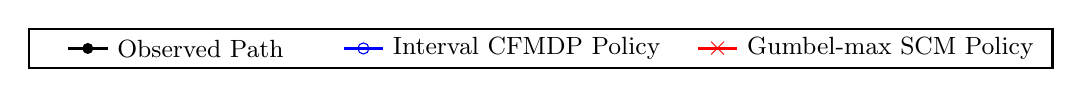
\begin{tikzpicture}[scale=1.0, every node/.style={scale=1.0}]
            \draw[thick, black] (-3, -0.25) rectangle (10, 0.25);
            %
            \draw[black, line width=1pt] (-2.5, 0.0) -- (-2,0.0);
            \fill[black] (-2.25,0.0) circle (2pt); %
            \node[right] at (-2,0.0) {\small Observed Path};
            
            %
            \draw[blue, line width=1pt] (1.0,0.0) -- (1.5,0.0);
            \node[draw=blue, circle, minimum size=4pt, inner sep=0pt] at (1.25,0.0) {}; %
            \node[right] at (1.5,0.0) {\small Interval CFMDP Policy};
            
            %
            \draw[red, line width=1pt] (5.5,0) -- (6,0);
            \node[red] at (5.75,0) {$\boldsymbol{\times}$}; %
            \node[right] at (6,0) {\small Gumbel-max SCM Policy};
        \end{tikzpicture}
    }\\
    %
    \subfigure[\footnotesize Lowest cumulative reward: Interval CFMDP ($312$), Gumbel-max SCM ($312$)]{%
        \resizebox{0.76\columnwidth}{!}{
             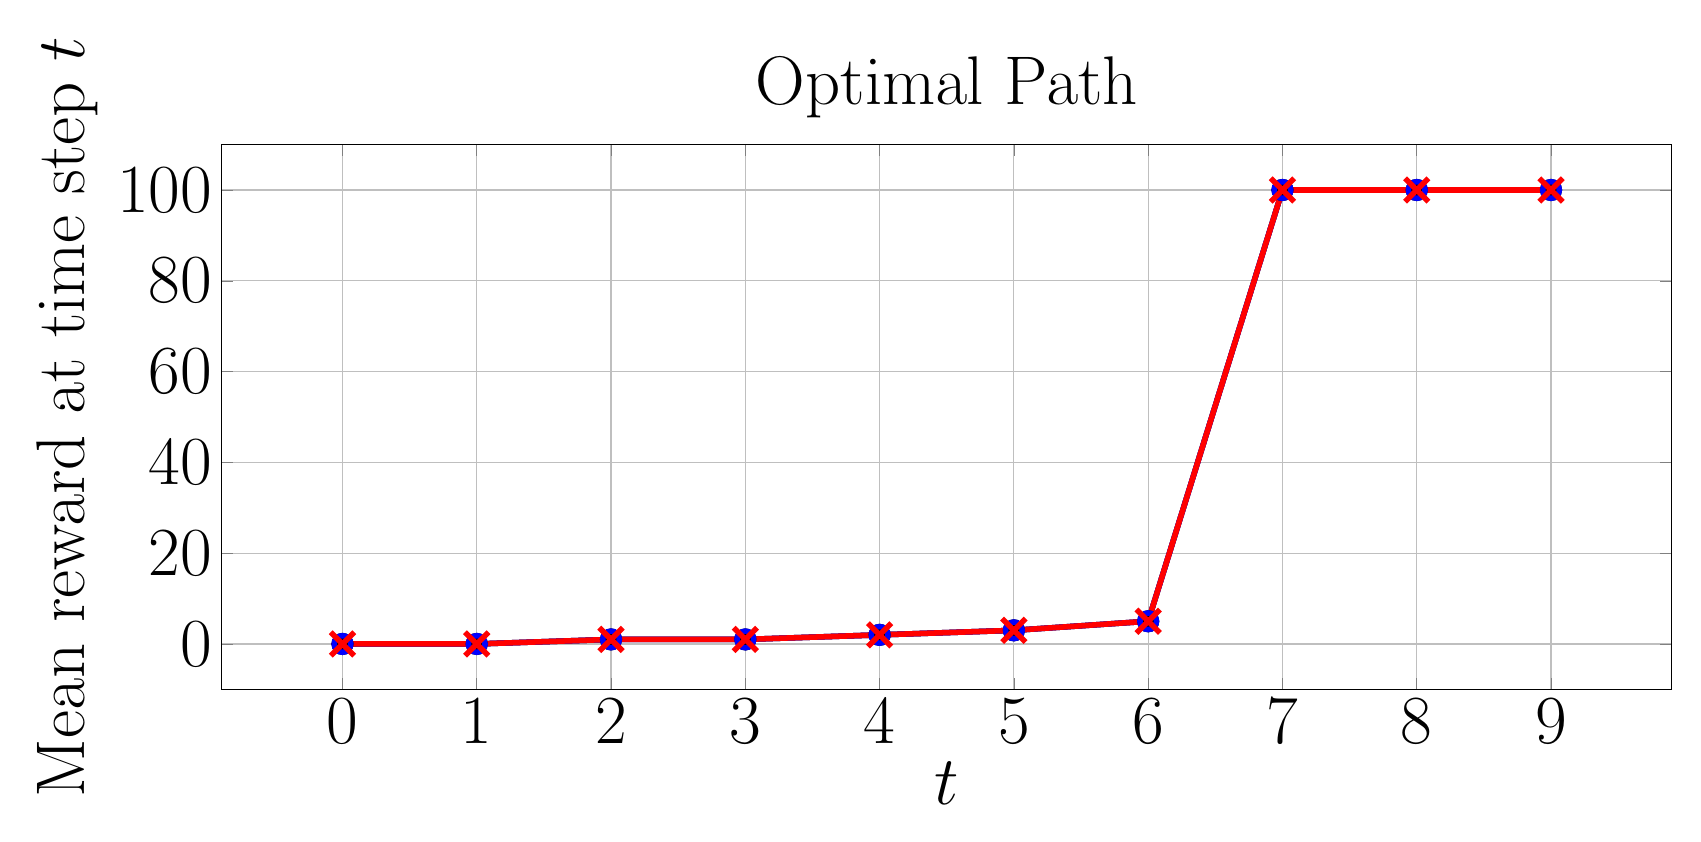
\begin{tikzpicture}
                \begin{axis}[
                    xlabel={$t$},
                    ylabel={Mean reward at time step $t$},
                    title={Optimal Path},
                    grid=both,
                    width=20cm, height=8.5cm,
                    every axis/.style={font=\Huge},
                    %
                ]
                \addplot[
                    color=black, %
                    mark=*, %
                    line width=2pt,
                    mark size=3pt,
                    error bars/.cd,
                    y dir=both, %
                    y explicit, %
                    error bar style={line width=1pt,solid},
                    error mark options={line width=1pt,mark size=4pt,rotate=90}
                ]
                coordinates {
                    (0, 0.0)  +- (0, 0.0)
                    (1, 0.0)  +- (0, 0.0) 
                    (2, 1.0)  +- (0, 0.0) 
                    (3, 1.0)  +- (0, 0.0)
                    (4, 2.0)  +- (0, 0.0)
                    (5, 3.0) +- (0, 0.0)
                    (6, 5.0) +- (0, 0.0)
                    (7, 100.0) +- (0, 0.0)
                    (8, 100.0) +- (0, 0.0)
                    (9, 100.0) +- (0, 0.0)
                };
                %
                \addplot[
                    color=blue, %
                    mark=o, %
                    line width=2pt,
                    mark size=3pt,
                    error bars/.cd,
                    y dir=both, %
                    y explicit, %
                    error bar style={line width=1pt,solid},
                    error mark options={line width=1pt,mark size=4pt,rotate=90}
                ]
                 coordinates {
                    (0, 0.0)  +- (0, 0.0)
                    (1, 0.0)  +- (0, 0.0) 
                    (2, 1.0)  +- (0, 0.0) 
                    (3, 1.0)  +- (0, 0.0)
                    (4, 2.0)  +- (0, 0.0)
                    (5, 3.0) +- (0, 0.0)
                    (6, 5.0) +- (0, 0.0)
                    (7, 100.0) +- (0, 0.0)
                    (8, 100.0) +- (0, 0.0)
                    (9, 100.0) +- (0, 0.0)
                };
                %
                \addplot[
                    color=red, %
                    mark=x, %
                    line width=2pt,
                    mark size=6pt,
                    error bars/.cd,
                    y dir=both, %
                    y explicit, %
                    error bar style={line width=1pt,solid},
                    error mark options={line width=1pt,mark size=4pt,rotate=90}
                ]
                coordinates {
                    (0, 0.0)  +- (0, 0.0)
                    (1, 0.0)  +- (0, 0.0) 
                    (2, 1.0)  +- (0, 0.0) 
                    (3, 1.0)  +- (0, 0.0)
                    (4, 2.0)  +- (0, 0.0)
                    (5, 3.0) +- (0, 0.0)
                    (6, 5.0) +- (0, 0.0)
                    (7, 100.0) +- (0, 0.0)
                    (8, 100.0) +- (0, 0.0)
                    (9, 100.0) +- (0, 0.0)
                };
                \end{axis}
            \end{tikzpicture}
         }
    }
    \hspace{1cm}
    \subfigure[\footnotesize Lowest cumulative reward: Interval CFMDP ($19$), Gumbel-max SCM ($-88$)]{%
         \resizebox{0.76\columnwidth}{!}{
            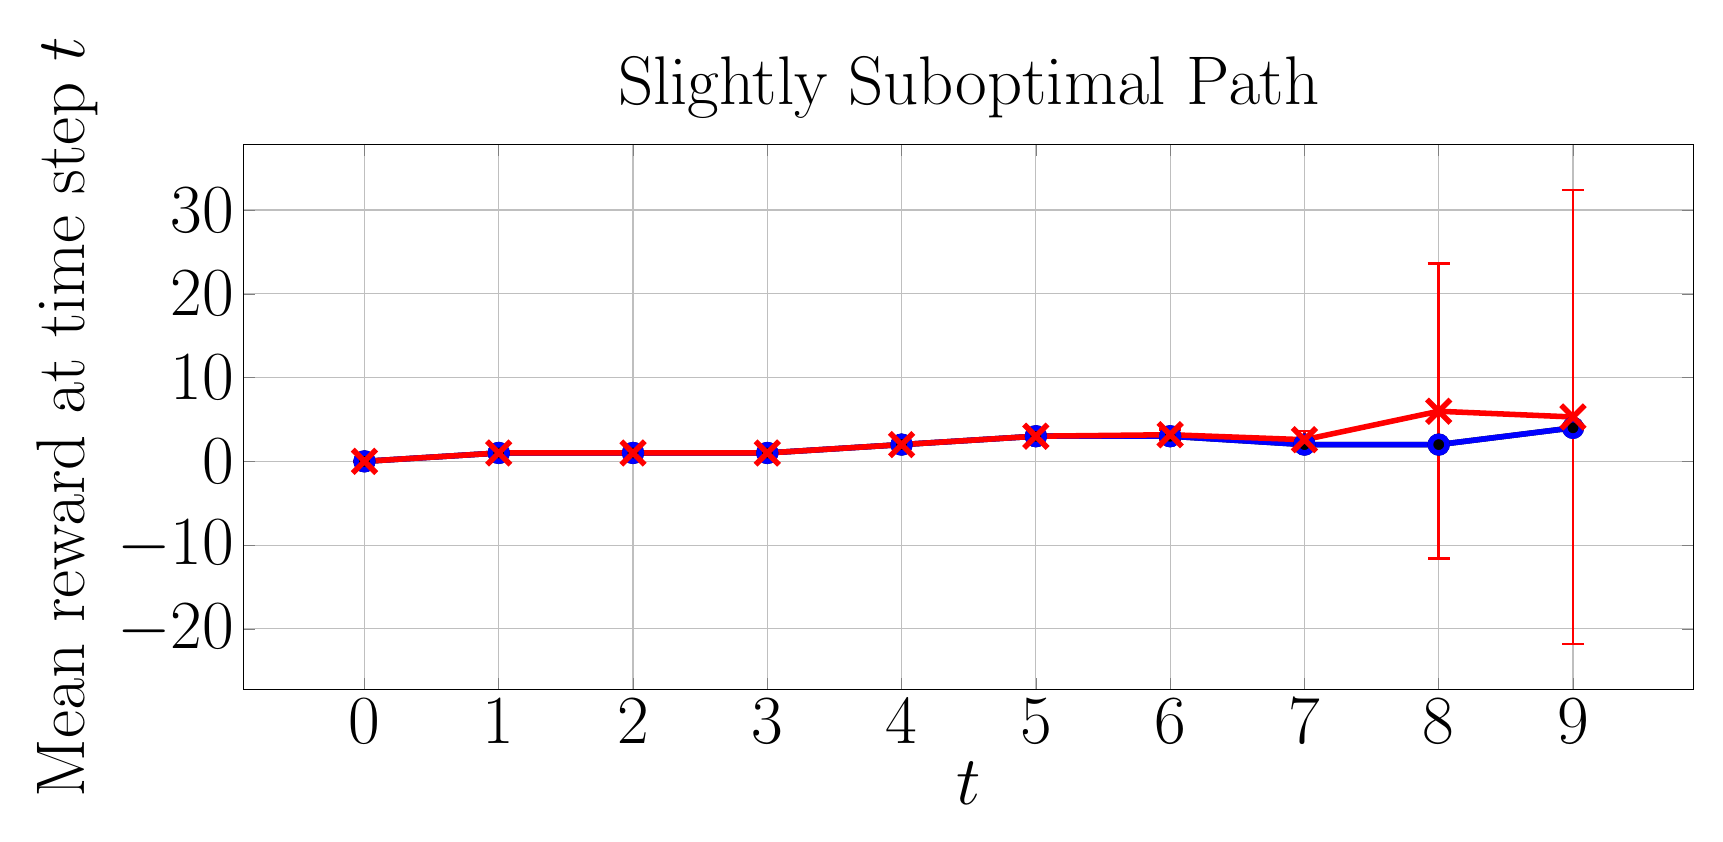
\begin{tikzpicture}
                \begin{axis}[
                    xlabel={$t$},
                    ylabel={Mean reward at time step $t$},
                    title={Slightly Suboptimal Path},
                    grid=both,
                    width=20cm, height=8.5cm,
                    every axis/.style={font=\Huge},
                    %
                ]
                \addplot[
                    color=black, %
                    mark=*, %
                    line width=2pt,
                    mark size=3pt,
                    error bars/.cd,
                    y dir=both, %
                    y explicit, %
                    error bar style={line width=1pt,solid},
                    error mark options={line width=1pt,mark size=4pt,rotate=90}
                ]
              coordinates {
                    (0, 0.0)  +- (0, 0.0)
                    (1, 1.0)  +- (0, 0.0) 
                    (2, 1.0)  +- (0, 0.0) 
                    (3, 1.0)  +- (0, 0.0)
                    (4, 2.0)  +- (0, 0.0)
                    (5, 3.0) +- (0, 0.0)
                    (6, 3.0) +- (0, 0.0)
                    (7, 2.0) +- (0, 0.0)
                    (8, 2.0) +- (0, 0.0)
                    (9, 4.0) +- (0, 0.0)
                };
                %
                \addplot[
                    color=blue, %
                    mark=o, %
                    line width=2pt,
                    mark size=3pt,
                    error bars/.cd,
                    y dir=both, %
                    y explicit, %
                    error bar style={line width=1pt,solid},
                    error mark options={line width=1pt,mark size=4pt,rotate=90}
                ]
              coordinates {
                    (0, 0.0)  +- (0, 0.0)
                    (1, 1.0)  +- (0, 0.0) 
                    (2, 1.0)  +- (0, 0.0) 
                    (3, 1.0)  +- (0, 0.0)
                    (4, 2.0)  +- (0, 0.0)
                    (5, 3.0) +- (0, 0.0)
                    (6, 3.0) +- (0, 0.0)
                    (7, 2.0) +- (0, 0.0)
                    (8, 2.0) +- (0, 0.0)
                    (9, 4.0) +- (0, 0.0)
                };
                %
                \addplot[
                    color=red, %
                    mark=x, %
                    line width=2pt,
                    mark size=6pt,
                    error bars/.cd,
                    y dir=both, %
                    y explicit, %
                    error bar style={line width=1pt,solid},
                    error mark options={line width=1pt,mark size=4pt,rotate=90}
                ]
                coordinates {
                    (0, 0.0)  +- (0, 0.0)
                    (1, 1.0)  +- (0, 0.0) 
                    (2, 1.0)  +- (0, 0.0) 
                    (3, 1.0)  +- (0, 0.0)
                    (4, 2.0)  += (0, 0.0)
                    (5, 3.0)  += (0, 0.0)
                    (6, 3.17847) += (0, 0.62606746) -= (0, 0.62606746)
                    (7, 2.5832885) += (0, 1.04598233) -= (0, 1.04598233)
                    (8, 5.978909) += (0, 17.60137623) -= (0, 17.60137623)
                    (9, 5.297059) += (0, 27.09227512) -= (0, 27.09227512)
                };
                \end{axis}
            \end{tikzpicture}
         }
    }\\[-1.5pt]
    \subfigure[\footnotesize Lowest cumulative reward: Interval CFMDP ($14$), Gumbel-max SCM ($-598$)]{%
         \resizebox{0.76\columnwidth}{!}{
             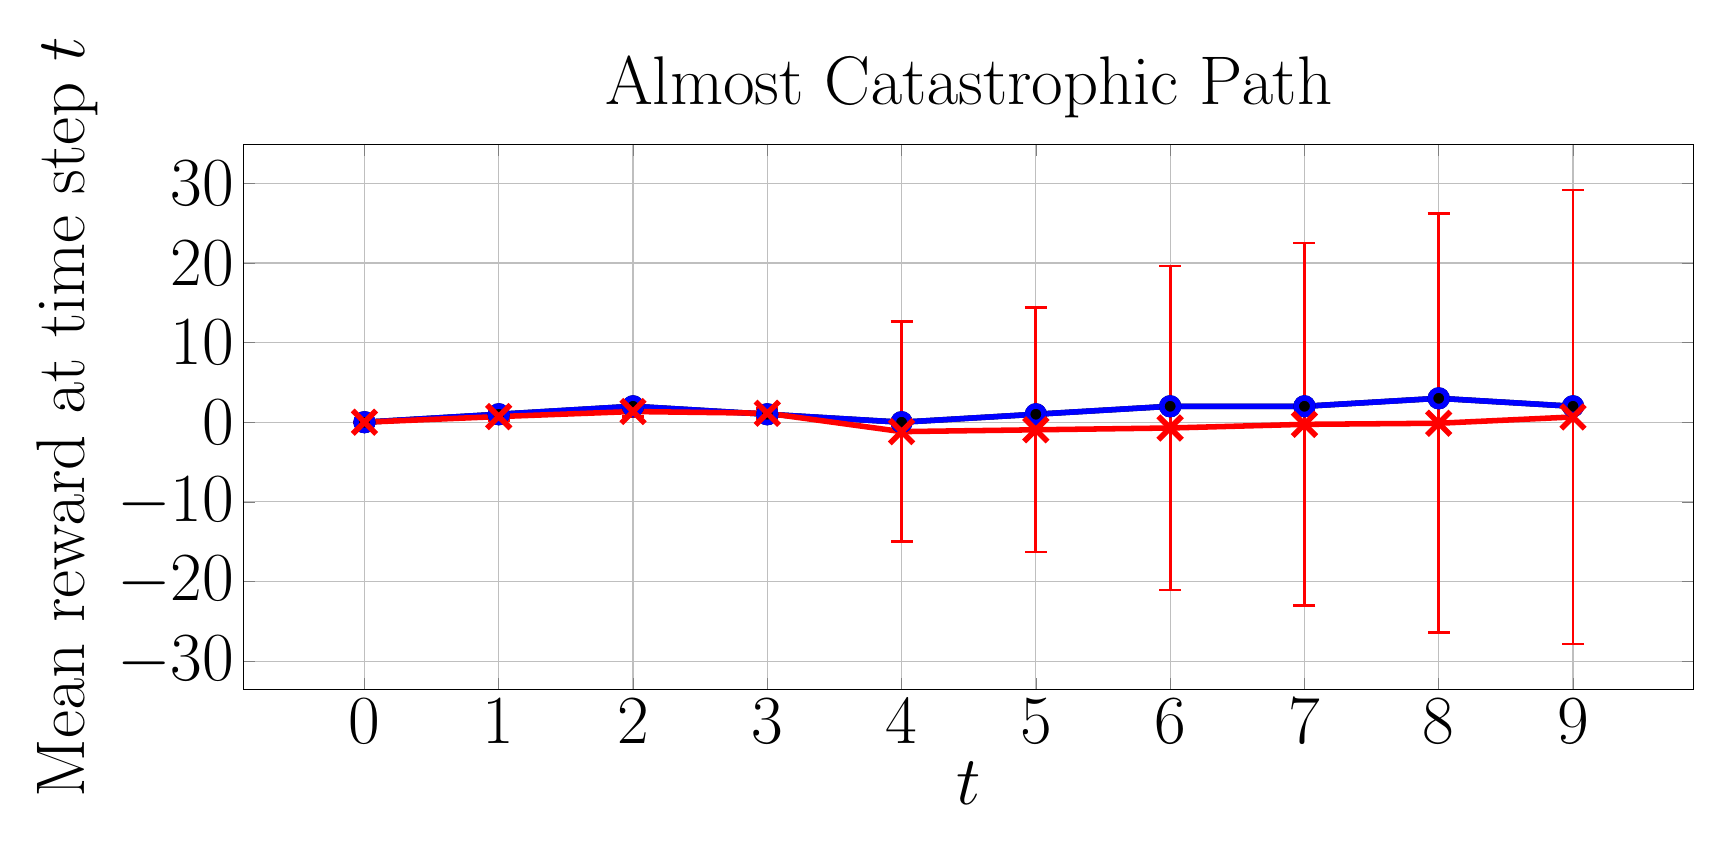
\begin{tikzpicture}
                \begin{axis}[
                    xlabel={$t$},
                    ylabel={Mean reward at time step $t$},
                    title={Almost Catastrophic Path},
                    grid=both,
                    width=20cm, height=8.5cm,
                    every axis/.style={font=\Huge},
                    %
                ]
                \addplot[
                    color=black, %
                    mark=*, %
                    line width=2pt,
                    mark size=3pt,
                    error bars/.cd,
                    y dir=both, %
                    y explicit, %
                    error bar style={line width=1pt,solid},
                    error mark options={line width=1pt,mark size=4pt,rotate=90}
                ]
                coordinates {
                    (0, 0.0)  +- (0, 0.0)
                    (1, 1.0)  +- (0, 0.0) 
                    (2, 2.0)  +- (0, 0.0) 
                    (3, 1.0)  +- (0, 0.0)
                    (4, 0.0)  +- (0, 0.0)
                    (5, 1.0) +- (0, 0.0)
                    (6, 2.0) +- (0, 0.0)
                    (7, 2.0) +- (0, 0.0)
                    (8, 3.0) +- (0, 0.0)
                    (9, 2.0) +- (0, 0.0)
                };
                %
                \addplot[
                    color=blue, %
                    mark=o, %
                    line width=2pt,
                    mark size=3pt,
                    error bars/.cd,
                    y dir=both, %
                    y explicit, %
                    error bar style={line width=1pt,solid},
                    error mark options={line width=1pt,mark size=4pt,rotate=90}
                ]
                coordinates {
                    (0, 0.0)  +- (0, 0.0)
                    (1, 1.0)  +- (0, 0.0) 
                    (2, 2.0)  +- (0, 0.0) 
                    (3, 1.0)  +- (0, 0.0)
                    (4, 0.0)  +- (0, 0.0)
                    (5, 1.0) +- (0, 0.0)
                    (6, 2.0) +- (0, 0.0)
                    (7, 2.0) +- (0, 0.0)
                    (8, 3.0) +- (0, 0.0)
                    (9, 2.0) +- (0, 0.0)
                };
                %
                \addplot[
                    color=red, %
                    mark=x, %
                    line width=2pt,
                    mark size=6pt,
                    error bars/.cd,
                    y dir=both, %
                    y explicit, %
                    error bar style={line width=1pt,solid},
                    error mark options={line width=1pt,mark size=4pt,rotate=90}
                ]
                coordinates {
                    (0, 0.0)  +- (0, 0.0)
                    (1, 0.7065655)  +- (0, 0.4553358) 
                    (2, 1.341673)  +- (0, 0.67091621) 
                    (3, 1.122926)  +- (0, 0.61281824)
                    (4, -1.1821935)  +- (0, 13.82444042)
                    (5, -0.952399)  +- (0, 15.35195457)
                    (6, -0.72672) +- (0, 20.33508414)
                    (7, -0.268983) +- (0, 22.77861454)
                    (8, -0.1310835) +- (0, 26.31013314)
                    (9, 0.65806) +- (0, 28.50670214)
                };
                %
            %
            %
            %
            %
            %
            %
            %
            %
            %
            %
            %
            %
            %
            %
            %
            %
            %
            %
                \end{axis}
            \end{tikzpicture}
         }
    }
    \hspace{1cm}
    \subfigure[\footnotesize Lowest cumulative reward: Interval CFMDP ($-698$), Gumbel-max SCM ($-698$)]{%
         \resizebox{0.76\columnwidth}{!}{
            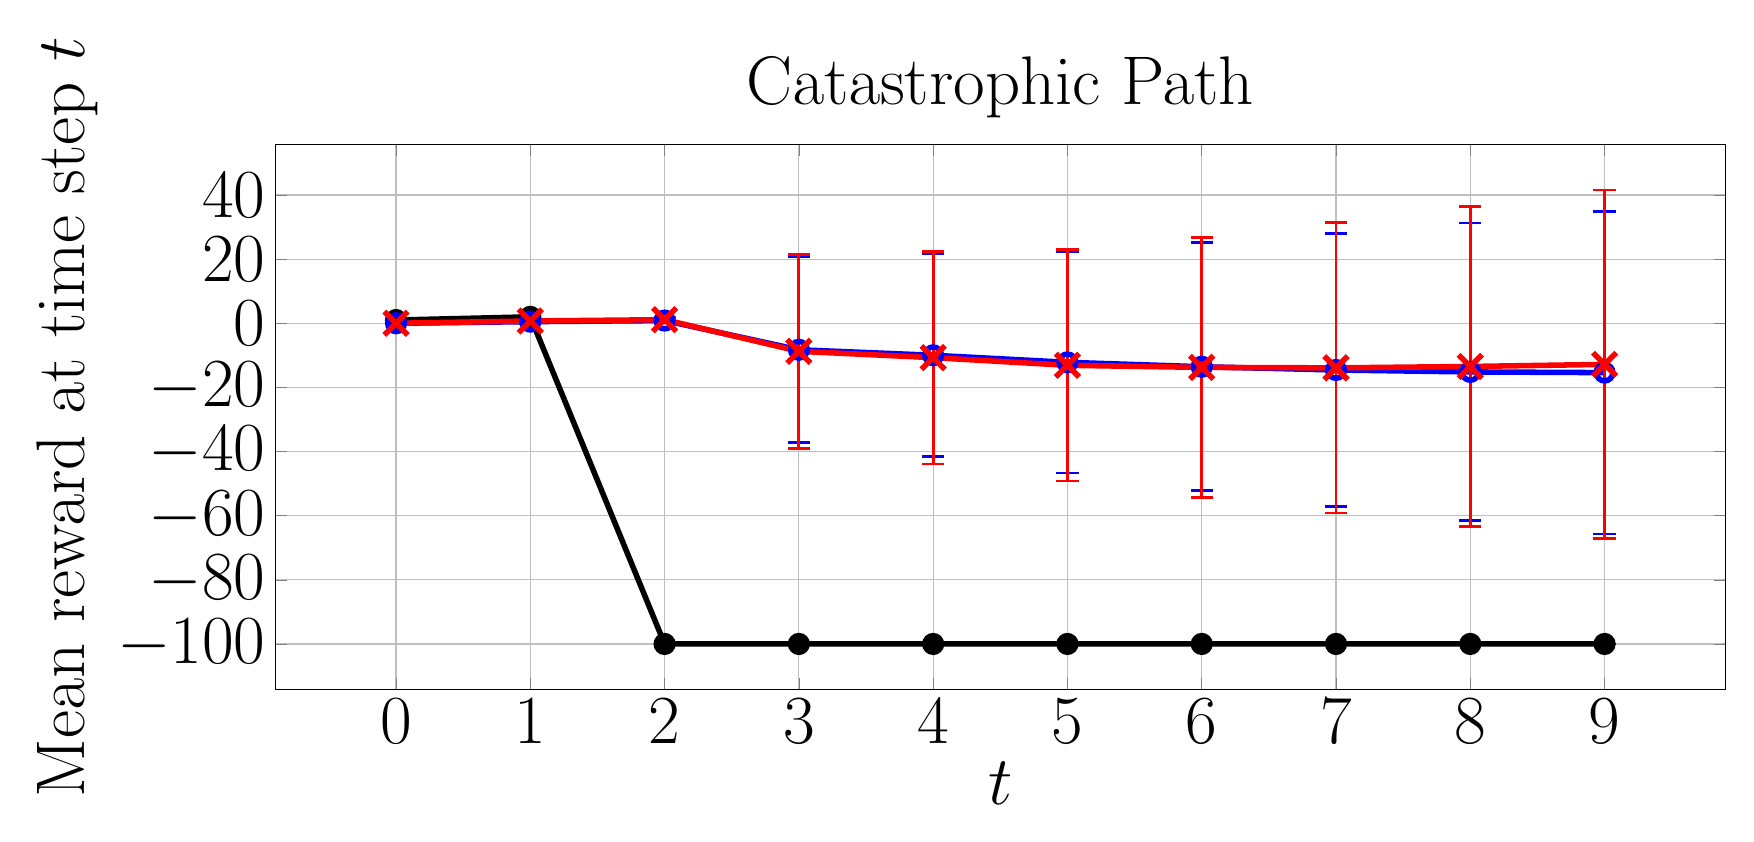
\begin{tikzpicture}
                \begin{axis}[
                    xlabel={$t$},
                    ylabel={Mean reward at time step $t$},
                    title={Catastrophic Path},
                    grid=both,
                    width=20cm, height=8.5cm,
                    every axis/.style={font=\Huge},
                    %
                ]
                \addplot[
                    color=black, %
                    mark=*, %
                    line width=2pt,
                    mark size=3pt,
                    error bars/.cd,
                    y dir=both, %
                    y explicit, %
                    error bar style={line width=1pt,solid},
                    error mark options={line width=1pt,mark size=4pt,rotate=90}
                ]
                coordinates {
                    (0, 1.0)  +- (0, 0.0)
                    (1, 2.0)  +- (0, 0.0) 
                    (2, -100.0)  +- (0, 0.0) 
                    (3, -100.0)  +- (0, 0.0)
                    (4, -100.0)  +- (0, 0.0)
                    (5, -100.0) +- (0, 0.0)
                    (6, -100.0) +- (0, 0.0)
                    (7, -100.0) +- (0, 0.0)
                    (8, -100.0) +- (0, 0.0)
                    (9, -100.0) +- (0, 0.0)
                };
                %
                \addplot[
                    color=blue, %
                    mark=o, %
                    line width=2pt,
                    mark size=3pt,
                    error bars/.cd,
                    y dir=both, %
                    y explicit, %
                    error bar style={line width=1pt,solid},
                    error mark options={line width=1pt,mark size=4pt,rotate=90}
                ]
                coordinates {
                    (0, 0.0)  +- (0, 0.0)
                    (1, 0.504814)  +- (0, 0.49997682) 
                    (2, 0.8439835)  +- (0, 0.76831917) 
                    (3, -8.2709165)  +- (0, 28.93656754)
                    (4, -9.981082)  +- (0, 31.66825363)
                    (5, -12.1776325) +- (0, 34.53463233)
                    (6, -13.556076) +- (0, 38.62845372)
                    (7, -14.574418) +- (0, 42.49603359)
                    (8, -15.1757075) +- (0, 46.41913968)
                    (9, -15.3900395) +- (0, 50.33563368)
                };
                %
                \addplot[
                    color=red, %
                    mark=x, %
                    line width=2pt,
                    mark size=6pt,
                    error bars/.cd,
                    y dir=both, %
                    y explicit, %
                    error bar style={line width=1pt,solid},
                    error mark options={line width=1pt,mark size=4pt,rotate=90}
                ]
                coordinates {
                    (0, 0.0)  +- (0, 0.0)
                    (1, 0.701873)  +- (0, 0.45743556) 
                    (2, 1.1227805)  +- (0, 0.73433129) 
                    (3, -8.7503255)  +- (0, 30.30257976)
                    (4, -10.722092)  +- (0, 33.17618589)
                    (5, -13.10721)  +- (0, 36.0648089)
                    (6, -13.7631645) +- (0, 40.56553451)
                    (7, -13.909043) +- (0, 45.23829402)
                    (8, -13.472517) +- (0, 49.96270296)
                    (9, -12.8278835) +- (0, 54.38618735)
                };
                %
            %
            %
            %
            %
            %
            %
            %
            %
            %
            %
            %
            %
            %
            %
            %
            %
            %
            %
                \end{axis}
            \end{tikzpicture}
         }
    }
    \caption{Average instant reward of CF paths induced by policies on GridWorld $p=0.4$.}
    \label{fig: reward p=0.4}
\end{figure*}

\subsection{Experimental Setup}
To compare policy performance, we measure the average rewards of counterfactual paths induced by our policy and the Gumbel-max policy by uniformly sampling $200$ counterfactual MDPs from the ICFMDP and generating $10,000$ counterfactual paths over each sampled CFMDP. \jl{Since the interval CFMDP depends on the observed path, we select $4$  paths of varying optimality to evaluate how the observed path impacts the performance of both policies: an optimal path, a slightly suboptimal path that could reach the optimal reward with a few changes, a catastrophic path that enters a catastrophic, terminal state with low reward, and an almost catastrophic path that was close to entering a catastrophic state.} When measuring the average probability bound widths and execution time needed to generate the ICFMDPs, we averaged over $20$ randomly generated observed paths
\footnote{Further training details are provided in Appendix \ref{app: training details}, and the code is provided at \href{https://github.com/ddv-lab/robust-cf-inference-in-MDPs}{https://github.com/ddv-lab/robust-cf-inference-in-MDPs}
%
%
.}.

\subsection{GridWorld}
\jl{The GridWorld MDP is a $4 \times 4$ grid where an agent must navigate from the top-left corner to the goal state in the bottom-right corner, avoiding a dangerous terminal state in the centre. At each time step, the agent can move up, down, left, or right, but there is a small probability (controlled by hyper-parameter $p$) of moving in an unintended direction. As the agent nears the goal, the reward for each state increases, culminating in a reward of $+100$ for reaching the goal. Entering the dangerous state results in a penalty of $-100$. We use two versions of GridWorld: a less stochastic version with $p=0.9$ (i.e., $90$\% chance of moving in the chosen direction) and a more stochastic version with $p=0.4$.}

\paragraph{GridWorld ($p=0.9$)}
When $p=0.9$, the counterfactual probability bounds are typically narrow (see Table \ref{tab:nonzero_probs} for average measurements). Consequently, as shown in Figure \ref{fig: reward p=0.9}, both policies are nearly identical and perform similarly well across the optimal, slightly suboptimal, and catastrophic paths.
%
However, for the almost catastrophic path, the interval CFMDP path is more conservative and follows the observed path more closely (as this is where the probability bounds are narrowest), which typically requires one additional step to reach the goal state than the Gumbel-max SCM policy.
%

\paragraph{GridWorld ($p=0.4$)}
\jl{When $p=0.4$, the GridWorld environment becomes more uncertain, increasing the risk of entering the dangerous state even if correct actions are chosen. Thus, as shown in Figure \ref{fig: reward p=0.4}, the interval CFMDP policy adopts a more conservative approach, avoiding deviation from the observed policy if it cannot guarantee higher counterfactual rewards (see the slightly suboptimal and almost catastrophic paths), whereas the Gumbel-max SCM is inconsistent: it can yield higher rewards, but also much lower rewards, reflected in the wide error bars.} For the catastrophic path, both policies must deviate from the observed path to achieve a higher reward and, in this case, perform similarly.
%
%
%
%
\subsection{Sepsis}
The Sepsis MDP \citep{oberst2019counterfactual} simulates trajectories of Sepsis patients. Each state consists of four vital signs (heart rate, blood pressure, oxygen concentration, and glucose levels), categorised as low, normal, or high.
and three treatments that can be toggled on/off at each time step (8 actions in total). Unlike \citet{oberst2019counterfactual}, we scale rewards based on the number of out-of-range vital signs, between $-1000$ (patient dies) and $1000$ (patient discharged). \jl{Like the GridWorld $p=0.4$ experiment, the Sepsis MDP is highly uncertain, as many states are equally likely to lead to optimal and poor outcomes. Thus, as shown in Figure \ref{fig: reward sepsis}, both policies follow the observed optimal and almost catastrophic paths to guarantee rewards are no worse than the observation.} However, improving the catastrophic path requires deviating from the observation. Here, the Gumbel-max SCM policy, on average, performs better than the interval CFMDP policy. But, since both policies have lower bounds clipped at $-1000$, neither policy reliably improves over the observation. In contrast, for the slightly suboptimal path, the interval CFMDP policy performs significantly better, shown by its higher lower bounds. 
Moreover, in these two cases, the worst-case counterfactual path generated by the interval CFMDP policy is better than that of the Gumbel-max SCM policy,
indicating its greater robustness.
%
\begin{figure*}
    \centering
     \resizebox{0.6\textwidth}{!}{
        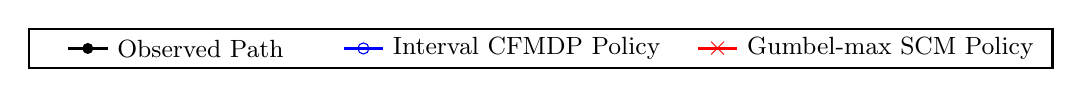
\begin{tikzpicture}[scale=1.0, every node/.style={scale=1.0}]
            \draw[thick, black] (-3, -0.25) rectangle (10, 0.25);
            %
            \draw[black, line width=1pt] (-2.5, 0.0) -- (-2,0.0);
            \fill[black] (-2.25,0.0) circle (2pt); %
            \node[right] at (-2,0.0) {\small Observed Path};
            
            %
            \draw[blue, line width=1pt] (1.0,0.0) -- (1.5,0.0);
            \node[draw=blue, circle, minimum size=4pt, inner sep=0pt] at (1.25,0.0) {}; %
            \node[right] at (1.5,0.0) {\small Interval CFMDP Policy};
            
            %
            \draw[red, line width=1pt] (5.5,0) -- (6,0);
            \node[red] at (5.75,0) {$\boldsymbol{\times}$}; %
            \node[right] at (6,0) {\small Gumbel-max SCM Policy};
        \end{tikzpicture}
    }\\
    \subfigure[\footnotesize Lowest cumulative reward: Interval CFMDP ($8000$), Gumbel-max SCM ($8000$)]{%
         \resizebox{0.76\columnwidth}{!}{
             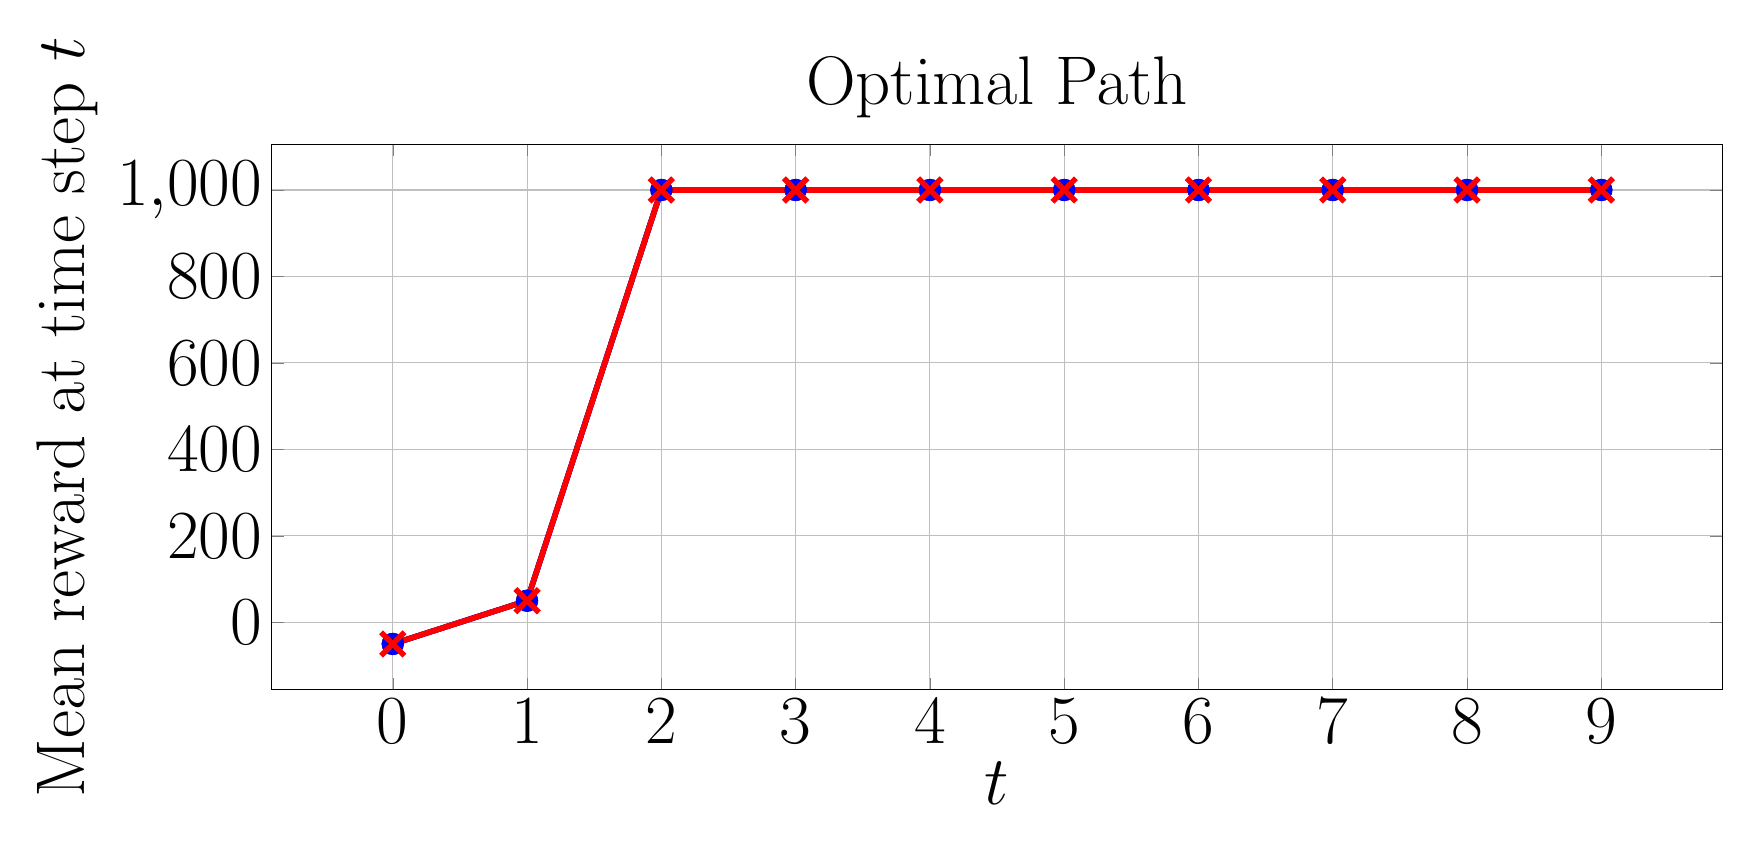
\begin{tikzpicture}
                \begin{axis}[
                    xlabel={$t$},
                    ylabel={Mean reward at time step $t$},
                    title={Optimal Path},
                    grid=both,
                    width=20cm, height=8.5cm,
                    every axis/.style={font=\Huge},
                    %
                ]
                \addplot[
                    color=black, %
                    mark=*, %
                    line width=2pt,
                    mark size=3pt,
                ]
                coordinates {
                    (0, -50.0)
                    (1, 50.0)
                    (2, 1000.0)
                    (3, 1000.0)
                    (4, 1000.0)
                    (5, 1000.0)
                    (6, 1000.0)
                    (7, 1000.0)
                    (8, 1000.0)
                    (9, 1000.0)
                };
                %
                \addplot[
                    color=blue, %
                    mark=o, %
                    line width=2pt,
                    mark size=3pt,
                    error bars/.cd,
                    y dir=both, %
                    y explicit, %
                    error bar style={line width=1pt,solid},
                    error mark options={line width=1pt,mark size=4pt,rotate=90}
                ]
                coordinates {
                    (0, -50.0)  +- (0, 0.0)
                    (1, 50.0)  +- (0, 0.0) 
                    (2, 1000.0)  +- (0, 0.0) 
                    (3, 1000.0)  +- (0, 0.0)
                    (4, 1000.0)  +- (0, 0.0)
                    (5, 1000.0) +- (0, 0.0)
                    (6, 1000.0) +- (0, 0.0)
                    (7, 1000.0) +- (0, 0.0)
                    (8, 1000.0) +- (0, 0.0)
                    (9, 1000.0) +- (0, 0.0)
                };
                %
                \addplot[
                    color=red, %
                    mark=x, %
                    line width=2pt,
                    mark size=6pt,
                    error bars/.cd,
                    y dir=both, %
                    y explicit, %
                    error bar style={line width=1pt,solid},
                    error mark options={line width=1pt,mark size=4pt,rotate=90}
                ]
                coordinates {
                    (0, -50.0)  +- (0, 0.0)
                    (1, 50.0)  +- (0, 0.0) 
                    (2, 1000.0)  +- (0, 0.0) 
                    (3, 1000.0)  +- (0, 0.0)
                    (4, 1000.0)  +- (0, 0.0)
                    (5, 1000.0) +- (0, 0.0)
                    (6, 1000.0) +- (0, 0.0)
                    (7, 1000.0) +- (0, 0.0)
                    (8, 1000.0) +- (0, 0.0)
                    (9, 1000.0) +- (0, 0.0)
                };
                %
                \end{axis}
            \end{tikzpicture}
         }
    }
    \hspace{1cm}
    \subfigure[\footnotesize Lowest cumulative reward: Interval CFMDP ($-5980$), Gumbel-max SCM ($-8000$)]{%
         \resizebox{0.76\columnwidth}{!}{
            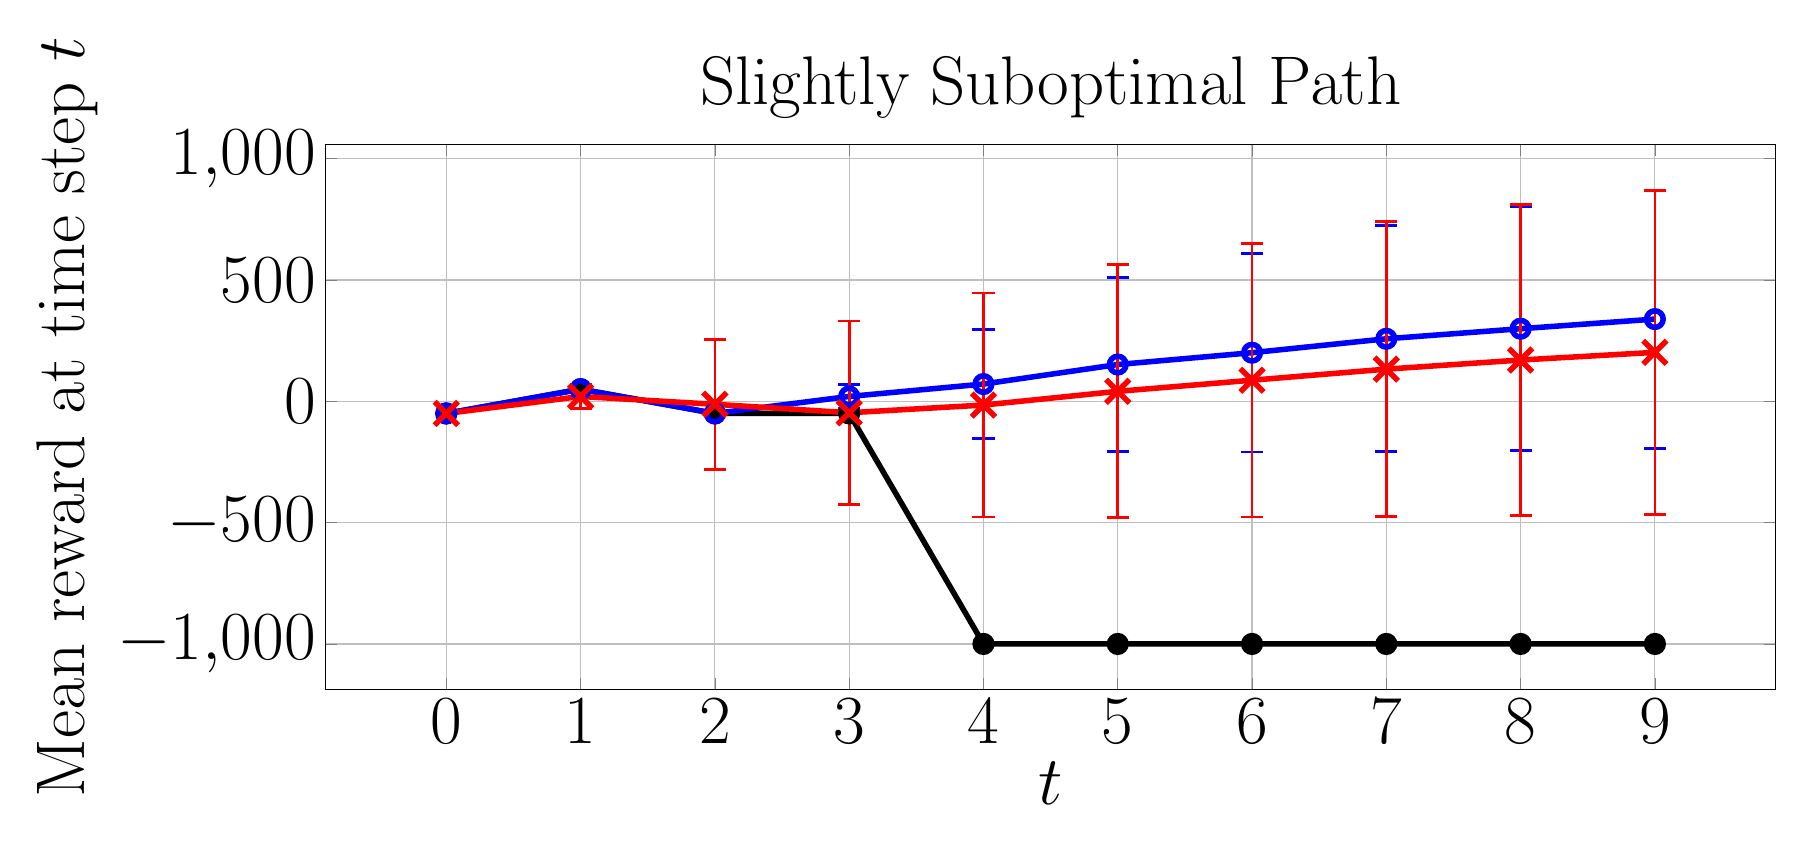
\begin{tikzpicture}
                \begin{axis}[
                    xlabel={$t$},
                    ylabel={Mean reward at time step $t$},
                    title={Slightly Suboptimal Path},
                    grid=both,
                    width=20cm, height=8.5cm,
                    every axis/.style={font=\Huge},
                    %
                ]
               \addplot[
                    color=black, %
                    mark=*, %
                    line width=2pt,
                    mark size=3pt,
                ]
                coordinates {
                    (0, -50.0)
                    (1, 50.0)
                    (2, -50.0)
                    (3, -50.0)
                    (4, -1000.0)
                    (5, -1000.0)
                    (6, -1000.0)
                    (7, -1000.0)
                    (8, -1000.0)
                    (9, -1000.0)
                };
                %
                \addplot[
                    color=blue, %
                    mark=o, %
                    line width=2pt,
                    mark size=3pt,
                    error bars/.cd,
                    y dir=both, %
                    y explicit, %
                    error bar style={line width=1pt,solid},
                    error mark options={line width=1pt,mark size=4pt,rotate=90}
                ]
                coordinates {
                    (0, -50.0)  +- (0, 0.0)
                    (1, 50.0)  +- (0, 0.0) 
                    (2, -50.0)  +- (0, 0.0) 
                    (3, 20.0631)  +- (0, 49.97539413)
                    (4, 71.206585)  +- (0, 226.02033693)
                    (5, 151.60797) +- (0, 359.23292559)
                    (6, 200.40593) +- (0, 408.86185176)
                    (7, 257.77948) +- (0, 466.10372804)
                    (8, 299.237465) +- (0, 501.82579506)
                    (9, 338.9129) +- (0, 532.06124996)
                };
                %
                \addplot[
                    color=red, %
                    mark=x, %
                    line width=2pt,
                    mark size=6pt,
                    error bars/.cd,
                    y dir=both, %
                    y explicit, %
                    error bar style={line width=1pt,solid},
                    error mark options={line width=1pt,mark size=4pt,rotate=90}
                ]
                coordinates {
                    (0, -50.0)  +- (0, 0.0)
                    (1, 20.00736)  +- (0, 49.99786741) 
                    (2, -12.282865)  +- (0, 267.598755) 
                    (3, -47.125995)  +- (0, 378.41755832)
                    (4, -15.381965)  +- (0, 461.77616558)
                    (5, 41.15459) +- (0, 521.53189262)
                    (6, 87.01595) +- (0, 564.22243126 )
                    (7, 132.62376) +- (0, 607.31338037)
                    (8, 170.168145) +- (0, 641.48013693)
                    (9, 201.813135) +- (0, 667.29441777)
                };
                %
                %
                %
                %
                %
                %
                %
                %
                %
                %
                %
                %
                %
                %
                %
                %
                %
                %
                %
                \end{axis}
            \end{tikzpicture}
         }
    }\\[-1.5pt]
    \subfigure[\footnotesize Lowest cumulative reward: Interval CFMDP ($100$), Gumbel-max SCM ($100$)]{%
         \resizebox{0.76\columnwidth}{!}{
             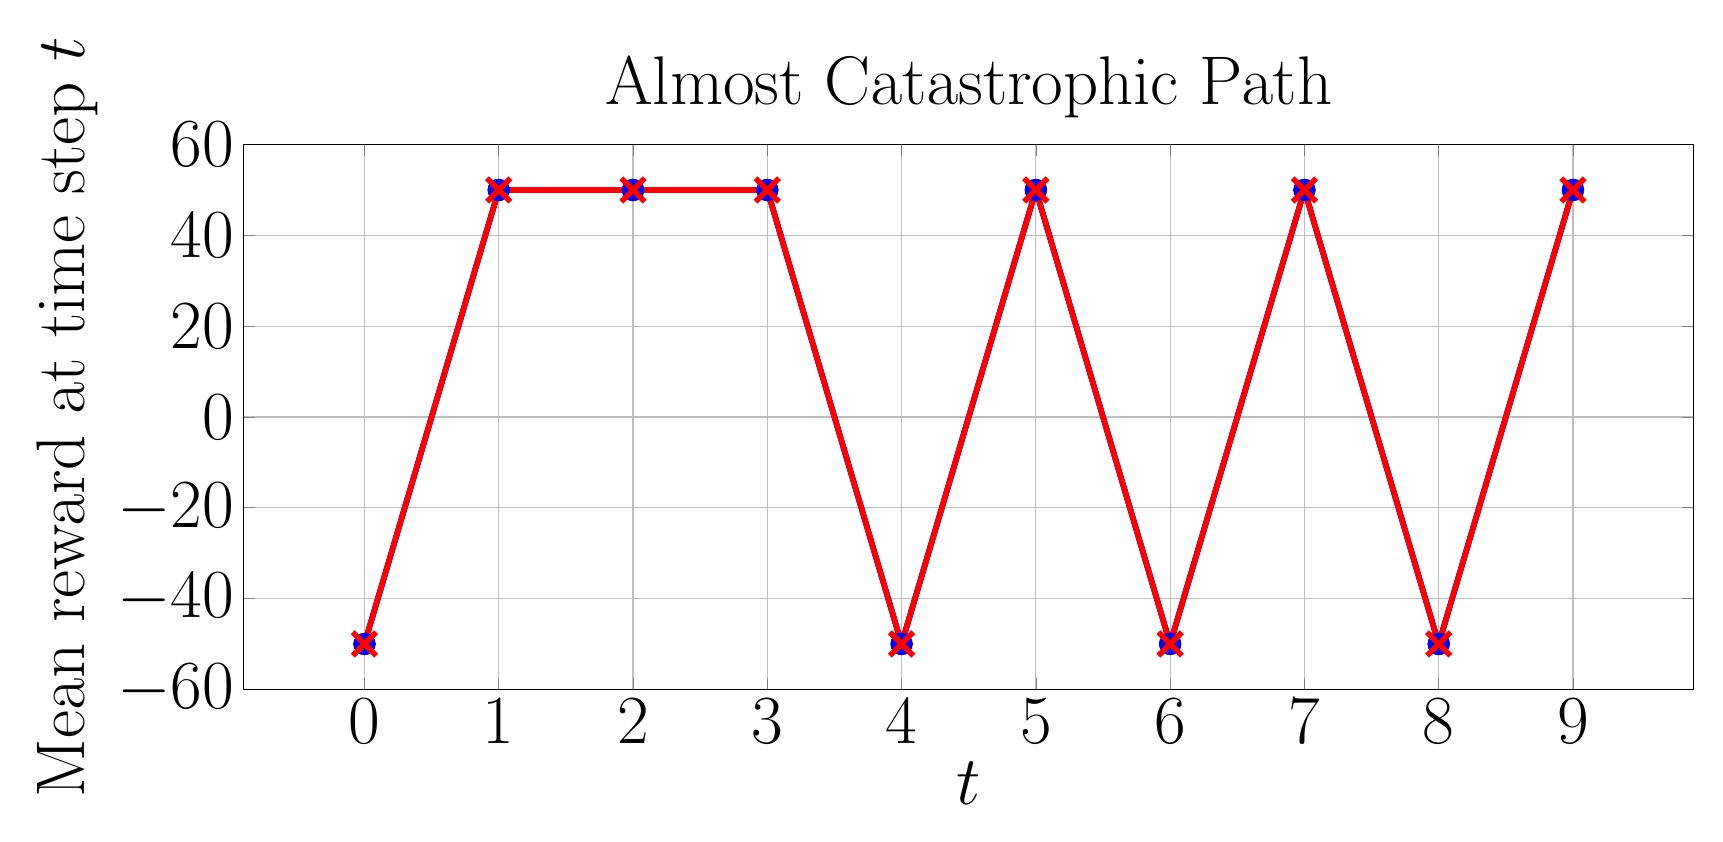
\begin{tikzpicture}
                \begin{axis}[
                    xlabel={$t$},
                    ylabel={Mean reward at time step $t$},
                    title={Almost Catastrophic Path},
                    grid=both,
                    every axis/.style={font=\Huge},
                    width=20cm, height=8.5cm,
                    %
                ]
               \addplot[
                    color=black, %
                    mark=*, %
                    line width=2pt,
                    mark size=3pt,
                ]
                coordinates {
                    (0, -50.0)
                    (1, 50.0)
                    (2, 50.0)
                    (3, 50.0)
                    (4, -50.0)
                    (5, 50.0)
                    (6, -50.0)
                    (7, 50.0)
                    (8, -50.0)
                    (9, 50.0)
                };
                %
                %
                \addplot[
                    color=blue, %
                    mark=o, %
                    line width=2pt,
                    mark size=3pt,
                    error bars/.cd,
                    y dir=both, %
                    y explicit, %
                    error bar style={line width=1pt,solid},
                    error mark options={line width=1pt,mark size=4pt,rotate=90}
                ]
                coordinates {
                    (0, -50.0)  +- (0, 0.0)
                    (1, 50.0)  +- (0, 0.0) 
                    (2, 50.0)  +- (0, 0.0) 
                    (3, 50.0)  +- (0, 0.0)
                    (4, -50.0)  +- (0, 0.0)
                    (5, 50.0) +- (0, 0.0)
                    (6, -50.0) +- (0, 0.0)
                    (7, 50.0) +- (0, 0.0)
                    (8, -50.0) +- (0, 0.0)
                    (9, 50.0) +- (0, 0.0)
                };
                %
                \addplot[
                    color=red, %
                    mark=x, %
                    line width=2pt,
                    mark size=6pt,
                    error bars/.cd,
                    y dir=both, %
                    y explicit, %
                    error bar style={line width=1pt,solid},
                    error mark options={line width=1pt,mark size=4pt,rotate=90}
                ]
                coordinates {
                    (0, -50.0)  +- (0, 0.0)
                    (1, 50.0)  +- (0, 0.0) 
                    (2, 50.0)  +- (0, 0.0) 
                    (3, 50.0)  +- (0, 0.0)
                    (4, -50.0)  +- (0, 0.0)
                    (5, 50.0) +- (0, 0.0)
                    (6, -50.0) +- (0, 0.0)
                    (7, 50.0) +- (0, 0.0)
                    (8, -50.0) +- (0, 0.0)
                    (9, 50.0) +- (0, 0.0)
                };
                %
                %
                %
                %
                %
                %
                %
                %
                %
                %
                %
                %
                %
                %
                %
                %
                %
                %
                %
                \end{axis}
            \end{tikzpicture}
         }
    }
    \hspace{1cm}
    \subfigure[\footnotesize Lowest cumulative reward: Interval CFMDP ($-7150$), Gumbel-max SCM ($-9050$)]{%
         \resizebox{0.76\columnwidth}{!}{
            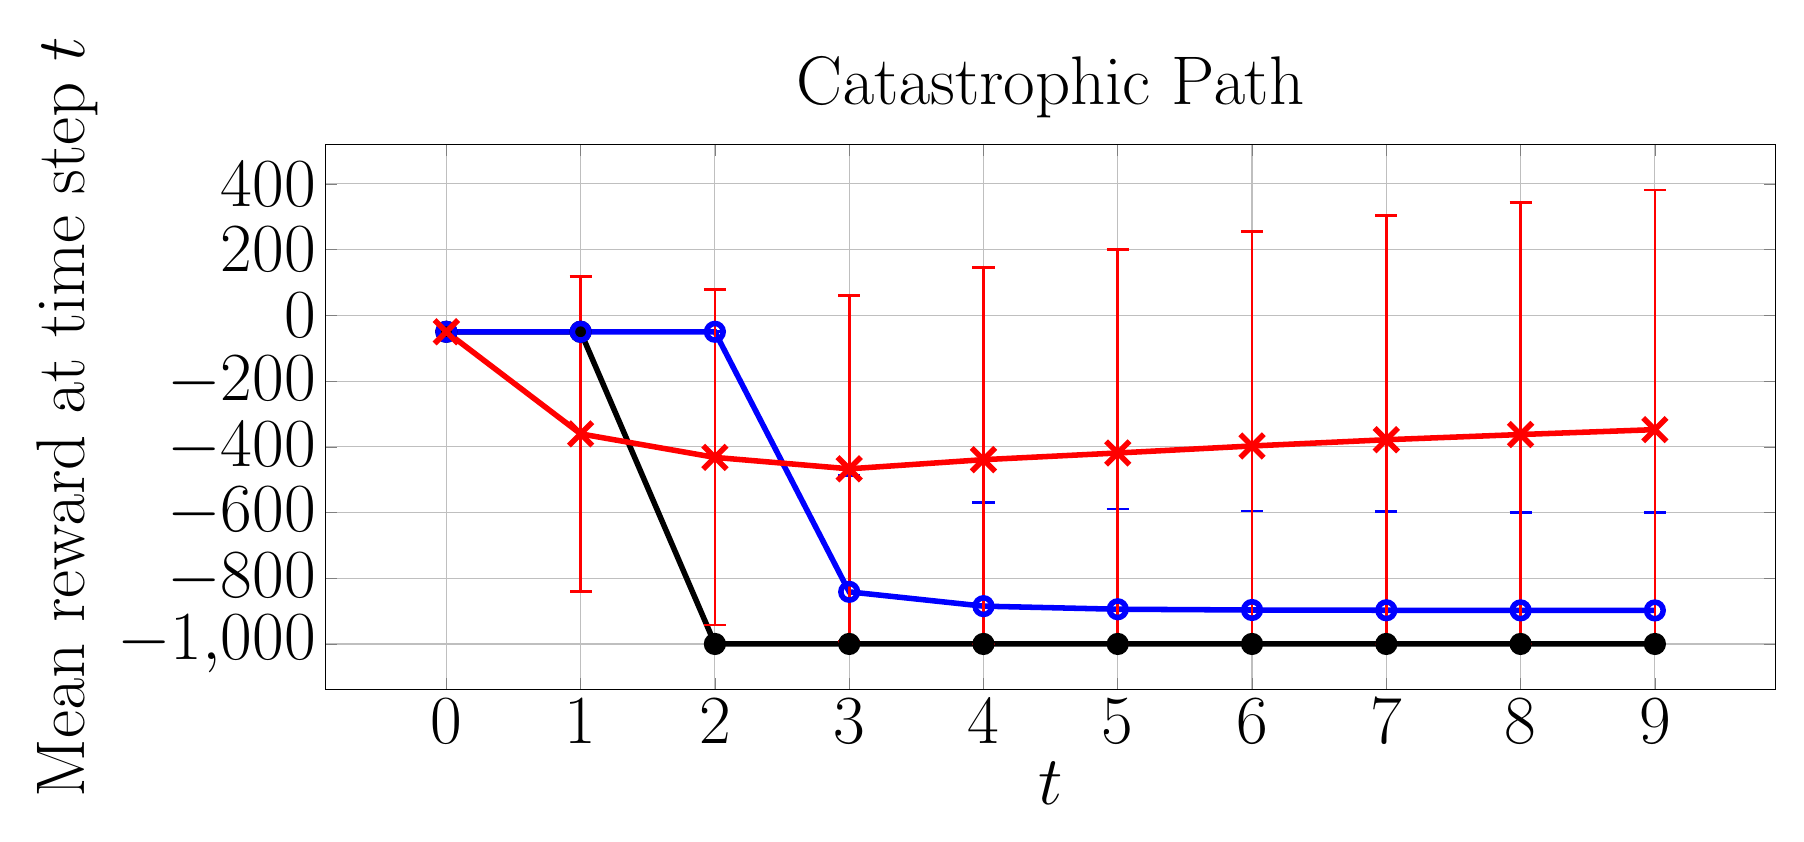
\begin{tikzpicture}
                \begin{axis}[
                    xlabel={$t$},
                    ylabel={Mean reward at time step $t$},
                    title={Catastrophic Path},
                    grid=both,
                    width=20cm, height=8.5cm,
                    every axis/.style={font=\Huge},
                    %
                ]
               \addplot[
                    color=black, %
                    mark=*, %
                    line width=2pt,
                    mark size=3pt,
                ]
                coordinates {
                    (0, -50.0)
                    (1, -50.0)
                    (2, -1000.0)
                    (3, -1000.0)
                    (4, -1000.0)
                    (5, -1000.0)
                    (6, -1000.0)
                    (7, -1000.0)
                    (8, -1000.0)
                    (9, -1000.0)
                };
                %
                %
                \addplot[
                    color=blue, %
                    mark=o, %
                    line width=2pt,
                    mark size=3pt,
                    error bars/.cd,
                    y dir=both, %
                    y explicit, %
                    error bar style={line width=1pt,solid},
                    error mark options={line width=1pt,mark size=4pt,rotate=90}
                ]
                coordinates {
                    (0, -50.0)  +- (0, 0.0)
                    (1, -50.0)  +- (0, 0.0) 
                    (2, -50.0)  +- (0, 0.0) 
                    (3, -841.440725)  += (0, 354.24605512) -= (0, 158.559275)
                    (4, -884.98225)  += (0, 315.37519669) -= (0, 115.01775)
                    (5, -894.330425) += (0, 304.88572805) -= (0, 105.669575)
                    (6, -896.696175) += (0, 301.19954514) -= (0, 103.303825)
                    (7, -897.4635) += (0, 299.61791279) -= (0, 102.5365)
                    (8, -897.77595) += (0, 298.80392585) -= (0, 102.22405)
                    (9, -897.942975) += (0, 298.32920557) -= (0, 102.057025)
                };
                %
                \addplot[
                    color=red, %
                    mark=x, %
                    line width=2pt,
                    mark size=6pt,
                    error bars/.cd,
                    y dir=both, %
                    y explicit, %
                    error bar style={line width=1pt,solid},
                    error mark options={line width=1pt,mark size=4pt,rotate=90}
                ]
            coordinates {
                    (0, -50.0)  +- (0, 0.0)
                    (1, -360.675265)  +- (0, 479.39812699) 
                    (2, -432.27629)  +- (0, 510.38620897) 
                    (3, -467.029545)  += (0, 526.36009628) -= (0, 526.36009628)
                    (4, -439.17429)  += (0, 583.96638919) -= (0, 560.82571)
                    (5, -418.82704) += (0, 618.43027478) -= (0, 581.17296)
                    (6, -397.464895) += (0, 652.67322574) -= (0, 602.535105)
                    (7, -378.49052) += (0, 682.85407033) -= (0, 621.50948)
                    (8, -362.654195) += (0, 707.01412023) -= (0, 637.345805)
                    (9, -347.737935) += (0, 729.29076479) -= (0, 652.262065)
                };
                %
                %
                %
                %
                %
                %
                %
                %
                %
                %
                %
                %
                %
                %
                %
                %
                %
                %
                %
                \end{axis}
            \end{tikzpicture}
         }
    }
    \caption{Average instant reward of CF paths induced by policies on Sepsis.}
    \label{fig: reward sepsis}
\end{figure*}

%
%
%
\subsection{Interval CFMDP Bounds}
%
%
Table \ref{tab:nonzero_probs} presents the mean counterfactual probability bound widths (excluding transitions where the upper bound is $0$) for each MDP, averaged over 20 observed paths. We compare the bounds under counterfactual stability (CS) and monotonicity (M) assumptions, CS alone, and no assumptions. This shows that the assumptions marginally reduce the bound widths, indicating the assumptions tighten the bounds without excluding too many causal models, as intended.
\renewcommand{\arraystretch}{1}

\begin{table}
\centering
\caption{Mean width of counterfactual probability bounds}
\resizebox{0.8\columnwidth}{!}{%
\begin{tabular}{|c|c|c|c|}
\hline
\multirow{2}{*}{\textbf{Environment}} & \multicolumn{3}{c|}{\textbf{Assumptions}} \\ \cline{2-4}
 & \textbf{CS + M} & \textbf{CS} & \textbf{None\tablefootnote{\jl{Equivalent to \citet{li2024probabilities}'s bounds (see Section \ref{sec: equivalence with Li}).}}} \\ \hline
\textbf{GridWorld} ($p=0.9$) & 0.0817 & 0.0977 & 0.100 \\ \hline
\textbf{GridWorld} ($p=0.4$) & 0.552  & 0.638  & 0.646 \\ \hline
\textbf{Sepsis} & 0.138 & 0.140 & 0.140 \\ \hline
\end{tabular}
}
\label{tab:nonzero_probs}
\end{table}


\subsection{Execution Times}
Table \ref{tab: times} compares the average time needed to generate the interval CFMDP vs.\ the Gumbel-max SCM CFMDP for 20 observations.
The GridWorld algorithms were run single-threaded, while the Sepsis experiments were run in parallel.
Generating the interval CFMDP is significantly faster as it uses exact analytical bounds, whereas the Gumbel-max CFMDP requires sampling from the Gumbel distribution to estimate counterfactual transition probabilities. \jl{Since constructing the counterfactual MDP models is the main bottleneck in both approaches, ours is more efficient overall and suitable for larger MDPs.}
\begin{table}
\centering
\caption{Mean execution time to generate CFMDPs}
\resizebox{0.99\columnwidth}{!}{%
\begin{tabular}{|c|c|c|}
\hline
\multirow{2}{*}{\textbf{Environment}} & \multicolumn{2}{c|}{\textbf{Mean Execution Time (s)}} \\ \cline{2-3} 
                                      & \textbf{Interval CFMDP} & \textbf{Gumbel-max CFMDP} \\ \hline
\textbf{GridWorld ($p=0.9$) }                  & 0.261                   & 56.1                      \\ \hline
\textbf{GridWorld ($p=0.4$)  }                 & 0.336                   & 54.5                      \\ \hline
\textbf{Sepsis}                                 & 688                     & 2940                      \\ \hline
\end{tabular}%
}
\label{tab: times}
\end{table}

\section{Software library for NVM data prefetching}
\label{sec:library}
\noindent The data readiness problem is likely to appear in any application that directly accesses large pools of data residing in NVM. In this section, we provide details on our general purpose data prefetching library, that aims to aid programmability to easily prefetch desired data regions. The library uses POSIX threads and implements a simple API to create, control and assign jobs to threads.

\subsection{Helper Threads}

Prefetching data~\cite{annavaram2001data} reduces the cache miss rate and hence
accelerates an application\textquotesingle s execution. An in-advance knowledge of memory regions
to be accessed can be used to prefetch data into caches before it is needed. However,
the application should not be stalled while prefetching the data. This can be achieved
by using independent helper threads for data prefetching.

Synchronization between the main computation thread and helper thread(s) is 
important~\cite{jung2006helper}. Prefetching data too early before it is needed
by the computation thread can result in cache pollution. Furthermore, required
cache lines may get evicted before they are accessed. Similarly, prefetching data
too late is also not useful, rather counter-productive. It can also lead to cache
pollution and degrade performance.

In our implementation, a helper thread is a simple block of code. Given a starting
memory address and the amount of data to be prefetched, the helper thread prefetches
data into caches without interfering with the main computation thread. We employ a
job queue to build a single producer - (multiple) consumer relationship between
a computation thread and one or multiple helper threads. We employ light-weight 
compare and swap instructions for synchronization in the job queue between a 
computation thread and the different helper threads.

A computation thread places the starting address and the amount of data to be prefetched into a job unit and enqueues it into the job queue. On the other end, a helper thread picks the job item, unpacks it and then prefetches the data into caches. Data prefetching is performed without stalling the computation thread.

\subsection{Library Services}
A programmer is responsible for inserting API calls to construct helper threads. However, as SE2 already has knowledge of the size and location of the block to be read, inserting data prefetching APIs in SE2 source code is not a tedious task. Our library provides three basic services via a simple API.

\begin{enumerate}%[leftmargin=*]
 \item \textbf{Creation of helper threads:} The library supports the  creation of a user-specified number of helper threads per computation thread, that are synchronized using a job queue. A slightly different thread creation policy is also supported, as explained in detail in Section 7.3.
 \item \textbf{Assigning work to helper threads:} Work is assigned to helper threads by placing jobs into their job queue. On arrival of a job into the queue, helper threads wake up, one fetches the job from the queue and starts the data prefetching. After completing the job, the helper thread again waits for the next job\textquotesingle s arrival if the queue is empty.
 \item \textbf{Mapping threads to cores:} Our library also supports the selection of a core (in a multicore platform) on which a particular helper thread is to be executed by setting thread affinities. The affinities can also be set with respect to the computational thread, i.e., selecting the same or a different core.
\end{enumerate}

\subsection{Thread Mapping Schemes for Our Case Study}
\label{sec:mapping-schemes}


\noindent As discussed in Section~\ref{sec:evaluation}, \emph{SE2} directly accesses data located in NVM disk, without copying it into any local buffer. This direct access results in high cache miss rates when the data is needed for processing. However, due to ad-hoc data prefetching, SE2 achieves performance improvements for a few queries (i.e., Q11, Q15,  and Q19), but not for the majority of them. By performing ad-hoc data prefetching we were able to prefetch some blocks into caches, but not most of them due to the overheads it entailed performing the prefetching inside the computation thread. Furthermore, ad-hoc placement of data prefetching in the source code of an application can be tedious and difficult to maintain.

By using our data prefetching library services, data can be brought closer to processing cores before 
it is needed. When accessing a file for a read operation, \emph{SE2} creates a memory mapping of the file 
using \verb+mmap()+. Additionally, it has knowledge of the location and size of the data block to be read. Therefore, \emph{SE2} can pack this information into a job and place it into the job queue to be processed by helper threads. By using this approach, PostgreSQL can continue with its computation while the required data is prefetched into caches by a helper thread. 

Due to the way PostgreSQL is structured, it is not necessary to have more than one helper thread active to service a queued job in time before the next arrives. Therefore, we propose two mappings that employ only one helper thread and a third mapping that employs a different thread creation policy by instantiating two helper threads that work in tandem as we explain in the following subsections.

\begin{figure*} %[htbp]
\centering     %%% not \center
\subfigure[\emph{M1} - Different physical core]{\label{CaseA}\includegraphics[width=32mm]{ThreadMapping_CaseA.eps}}
\subfigure[\emph{M2} - Same physical core (HT)]{\label{CaseB}\includegraphics[width=52mm]{ThreadMapping_CaseB.eps}}
\subfigure[\emph{M3} - Thread mapping for the two helper threads scheme]{\label{CaseE}\includegraphics[width=87mm]{ThreadMapping_CaseE.eps}}
\caption{Different Helper thread mapping schemes with and without hyper-threading (HT) enabled}
\label{Thread-Mapping}
\end{figure*}


\subsubsection{Single helper thread}



When using a single helper thread there are two options for thread mapping. Mapping it to a different core than that of the computation thread, or to the same core. The latter option makes sense if the target machine supports hyper-threading - i.e., two hardware thread contexts per core. We explore these thread mappings:
\begin{enumerate}
 \item \verb+M1+ - Map helper thread to a different physical core, as shown in Fig.~\ref{CaseA}. In this case, each thread resides in a different core and hence prefetching is not done at the level of private caches but at the level of the last level cache, which is shared across cores.
 \item \verb+M2+ - Map helper thread into the same physical core while making use of hyper-threading, as shown in Fig.~\ref{CaseB}. Both threads reside within the same physical core, hence prefetching will also populate the private L1 and L2 caches present in the core.
\end{enumerate}

\subsubsection{Two helper threads}

As described for case \emph{M2}, the helper thread prefetches data into the private caches of the core where the computation thread is executing. However, in this scenario, the helper thread competes with the computation thread for hardware resources. This competition can slow down the execution of the computation thread. On the other hand, for case \emph{M1} there is no such competition for hardware resources at the expense of prefetching into the LLC, further away from the processing core.

A good compromise can be achieved using two helper threads working together. One helper thread is mapped to a different physical core than that of the computation thread and will process the jobs enqueued by the computation thread, similar to case \emph{M1}. Once this first thread finishes processing the job, it enqueues the same job into a second job queue that is processed by the second helper thread that is mapped into the same physical core as the computation thread. This thread mapping scheme which we term \verb+M3+ is shown in Fig.~\ref{CaseE}. The rationale behind this proposal is that the high penalty miss from main memory to LLC will be paid by a different core, while the helper thread residing on the same core as the computation thread will put data into the private caches and complete jobs much faster since data will be already present in the LLC.

\section{Evaluation of the data prefetching library}
\label{sec:library-evalualtion}

\begin{figure*}
\centering
\includegraphics[width=\linewidth]{kernel-exec-percent-pg-new.eps}
\caption{Percentage of kernel execution time for PostgreSQL thread}
\label{kernel-time-pg}
\end{figure*}

\noindent In this section, we evaluate our modified storage engine \emph{SE2} while using the data prefetching library. 
For the scenarios in which we employ the library, we remove the simple ad-hoc software prefetching scheme used in the previous evaluation. However, the \emph{pmfs\_se2} system to which we compare does include the same ad-hoc prefetching used in the previous evaluation (Section~\ref{sec:evaluation}). The test machine and methodology employed is the same as explained in Section~\ref{sec:methodology}, with the exception that hyper-threading (HT) is enabled for \emph{M2} and \emph{M3}.



\subsection{Performance Impact on Kernel Execution Time}

Fig. \ref{kernel-time-pg} shows the percentage of kernel execution time of the PostgreSQL thread (computation thread) for each of the evaluated queries. As explained in Section~\ref{sec:evaluation}, \emph{SE2} only redirects the buffer pointer for file read operation from the local buffer cache to an NVM disk address that is within the address space of the PostgreSQL process. Hence, there is no data movement at the kernel level. As a result, the involvement of kernel in data movement and hence the average percentage of kernel execution time is already low in \emph{pmfs\_se2} as compared to \emph{pmfs\_base95}, reducing from 10\% to 3\%.

When using \verb+M1+, \verb+M2+, and \verb+M3+ helper thread schemes, by offloading the prefetching of entire blocks of data to helper threads, we can further hide kernel execution time overheads for the PostgreSQL thread running the query. Helper threads are more effective in prefetching data than the ad-hoc scheme used in pmfs\_se2. Therefore, the average percentage of kernel execution time further reduces from 3\% for \emph{pmfs\_se2} to 0.5\% in \verb+M1+, \verb+M2+, and \verb+M3+.

There is no noticeable difference between the three thread mapping schemes in terms of percentage of kernel execution time. The reason is that all three mapping schemes place data blocks at least into the LLC, which is enough to hide kernel related events such as page faults. 

\begin{figure*}
\centering
\includegraphics[width=\linewidth]{exec-time-new.eps}
\caption{Wall-clock execution time normalized with respect to pmfs\_base95}
\label{exec-time-new}
\end{figure*}
\begin{figure*}
\centering
\includegraphics[width=\linewidth]{compute-stall-pg.eps}
\caption{Execution time breakdown into compute and stall cycles for PostgreSQL thread, normalized with respect to pmfs\_base95}
\label{compute-stall-pg}
\end{figure*}

\subsection{Query Performance Improvement}\label{QPI}

Fig.~\ref{exec-time-new} shows the wall-clock query execution time normalized with respect to \emph{pmfs\_base95} for all queries. We can observe that for queries in which \emph{pmfs\_se2} obtained better performance, the new evaluated systems with our prefetch library overall obtain better execution times, especially for the \verb+M3+ thread mapping scheme. M3 shows noticeable performance improvements for queries where the sequential scan operation represents a significant fraction of the total database operations - i.e. Q03-Q12, Q15, and Q19, as shown in Fig. \ref{query-breakdown}. On the other hand, queries where sequential scan operation consume less time (i.e. Q01, Q02, Q13, Q17, and Q20), show no performance improvement. On average, M3 obtains an 8\% performance improvement over the baseline. \verb+M1+ and \verb+M2+ show up to 13\% performance improvement (Q11), with an average of 6\% when compared to pmfs\_base95. 

Query execution time is mostly affected by two factors: cache misses and competition for hardware resources between threads mapped on the same physical core. Reducing any of these two factors should lead to better query execution times. To understand the improvements seen in Fig.~\ref{exec-time-new}, we provide insights in terms of compute and stalled core cycles and L1 cache misses for the PostgreSQL thread in Fig.~\ref{compute-stall-pg} and Fig.~\ref{L1-misses-pg}, respectively.

\begin{figure*}
\centering
\includegraphics[width=\linewidth]{L1-misses-total.eps}
\caption{L1 cache misses for PostgreSQL thread normalized with respect to pmfs base95}
\label{L1-misses-pg}
\end{figure*}

Fig.~\ref{compute-stall-pg} shows an execution cycle break down into the stall and compute cycles for all evaluated queries, but just for the PostgreSQL thread. An execution cycle is classified as `compute', if at least one instruction is committed during that cycle, or as `stalled' otherwise. Both \verb+M1+ and \verb+M2+ generate similar results in terms of wall-clock execution time. In Fig.~\ref{compute-stall-pg}, we can observe that both are able to reduce the kernel stall and compute components due to less kernel involvement in the main computation thread since the prefetching and kernel related events such as page faults are handled by the helper thread. However, the user level components are still very similar. This is because, as shown in Fig.~\ref{L1-misses-pg}, the actual number of L1 cache misses is also similar despite helper threads prefetching at different levels of the memory hierarchy. We attribute this to hardware prefetchers being much more efficient once the data is already in the LLC. M3 shows better performance than M1 and M2 as it maps the helper-thread, which handles the page faults, on a core different than that of compute thread as shown in Fig. \ref{CaseE}. Nonetheless, Fig.~\ref{L1-misses-pg} shows a large L1 cache misses reduction when compared to both \emph{pmfs\_base95} and \emph{pmfs\_se2}, proving that the prefetching library is performing well in hiding them from the main computation thread.

We can see in Fig.~\ref{compute-stall-pg} that \verb+M3+, besides being able to reduce the kernel components, also reduces the time spent in stalled user significantly, e.g., in Q03, Q05, Q06, Q12, and others. This is because of two factors: (i) prefetching into the L1 cache with our library is more timely than hardware prefetching, which might still be in-flight when the data is actually needed; and (ii) by using the two thread mapping approach we are able to reduce the overhead of the helper thread that is sharing the same physical core with the computation thread. Therefore, the first helper thread in \verb+M3+ brings the data into the LLC without interfering with the PostgreSQL thread that is running on a different physical core. While the second thread running on the same core brings the data into the private caches while incurring a lower overhead due to lower latency misses.

\begin{figure*}
\centering
\includegraphics[width=\linewidth]{results_Helper1.eps}
\caption{Execution time breakdown into compute and stall cycles for 
helper thread running on same physical core as PostgreSQL in M2 and M3. Execution time is normalized with respect to M2}
\label{compute-stall-helper}
\end{figure*}

To support this explanation, Fig.~\ref{compute-stall-helper} shows the compute-stall cycle breakdown for the helper thread that shares the physical core with the computation PostgreSQL thread for \verb+M2+ and \verb+M3+ schemes. We can observe that for the queries in which \verb+M3+ performs better (e.g., Q03, Q05, Q06, and Q12), the helper thread sharing the core is more lightweight. In particular, the helper thread in \verb+M3+ does not suffer from kernel noise since the kernel related events like page faults are sorted by the other helper thread running on a different core, leading to a load reduction in the computation core. Also, a reduction in user stalled cycles can be observed (e.g., Q11 and Q15) due to lower latency memory accesses.

We find that our library is able to help improve the performance with little programming effort. The ad-hoc prefetching scheme used in \emph{pmfs\_se2}, while simple, still required code analysis to place the prefetch instructions in different places in order to maximize the number of data blocks prefetched without stalling too much the computations. With our library the creation and mapping of threads is done only once, and the creation of jobs to be enqueued came as a natural fit in a single point of the source code, i.e., when the needed block is memory mapped.

\section{Related Works}
\label{sec:rw}

%-------------------------------------------------------------------------
\noindent \textbf{Vision-Language Model.}
In recent years, vision-language models, as a novel tool capable of processing both visual and linguistic modalities, have garnered widespread attention. These models, such as CLIP~\cite{clip}, ALIGN~\cite{ALIGN}, BLIP~\cite{BLIP}, FILIP~\cite{filip}, etc., leverage self-supervised training on image-text pairs to establish connections between vision and text, enabling the models to comprehend image semantics and their corresponding textual descriptions. This powerful understanding allows vision-language models (e.g., CLIP) to exhibit remarkable generalization capabilities across various downstream tasks~\cite{downsteam1,downsteam2,downsteam3,h2b}. To further enhance the transferability of vision-language models to downstream tasks, prompt tuning and adapter methods have been applied. However, methods based on prompt tuning (such as CoOp~\cite{coop}, CoCoOp~\cite{cocoop}, Maple~\cite{maple}) and adapter-based methods (such as Tip-Adapter~\cite{tip}, CLIP-Adapter~\cite{clip_adapter}) often require large amounts of training data when transferring to downstream tasks, which conflicts with the need for rapid adaptation in real-world applications. Therefore, this paper focuses on test-time adaptation~\cite{tpt}, a method that enables transfer to downstream tasks without relying on training data.

%-------------------------------------------------------------------------
\noindent \textbf{Test-Time Adaptation.}
Test-time adaptation~(TTA) refers to the process by which a model quickly adapts to test data that exhibits distributional shifts~\cite{tta1,memo,ptta,domainadaptor,dota}. Specifically, it requires the model to handle these shifts in downstream tasks without access to training data. TPT~\cite{tpt} optimizes adaptive text prompts using the principle of entropy minimization, ensuring that the model produces consistent predictions for different augmentations of test images generated by AugMix~\cite{augmix}. DiffTPT~\cite{difftpt} builds on TPT by introducing the Stable Diffusion Model~\cite{stable} to create more diverse augmentations and filters these views based on their cosine similarity to the original image. However, both TPT and DiffTPT still rely on backpropagation to optimize text prompts, which limits their ability to meet the need for fast adaptation during test-time. TDA~\cite{tda}, on the other hand, introduces a cache model like Tip-Adapter~\cite{tip} that stores representative test samples. By comparing incoming test samples with those in the cache, TDA refines the model’s predictions without the need for backpropagation, allowing for test-time enhancement. Although TDA has made significant improvements in the TTA task, it still does not fundamentally address the impact of test data distribution shifts on the model and remains within the scope of CLIP's original feature space. We believe that in TTA tasks, instead of making decisions in the original space, it would be more effective to map the features to a different spherical space to achieve a better decision boundary.

%-------------------------------------------------------------------------
\noindent \textbf{Statistical Learning.}
Statistical learning techniques play an important role in dimensionality reduction and feature extraction. Support Vector Machines~(SVM)~\cite{svm} are primarily used for classification tasks but have been adapted for space mapping through their ability to create hyperplanes that separate data in high-dimensional spaces. The kernel trick enables SVM to operate in transformed feature spaces, effectively mapping non-linearly separable data. PCA~\cite{pca} is a linear transformation method that maps high-dimensional data to a new lower-dimensional space through a linear transformation, while preserving as much important information from the original data as possible.
\section{Conclusion}
In this work, we propose a simple yet effective approach, called SMILE, for graph few-shot learning with fewer tasks. Specifically, we introduce a novel dual-level mixup strategy, including within-task and across-task mixup, for enriching the diversity of nodes within each task and the diversity of tasks. Also, we incorporate the degree-based prior information to learn expressive node embeddings. Theoretically, we prove that SMILE effectively enhances the model's generalization performance. Empirically, we conduct extensive experiments on multiple benchmarks and the results suggest that SMILE significantly outperforms other baselines, including both in-domain and cross-domain few-shot settings.







%\section{Introduction}
%\label{intro}
%Your text comes here. Separate text sections with
%\section{Section title}
%\label{sec:1}
%Text with citations \cite{RefB} and \cite{RefJ}.
%\subsection{Subsection title}
%\label{sec:2}
%as required. Don't forget to give each section
%and subsection a unique label (see Sect.~\ref{sec:1}).
%\paragraph{Paragraph headings} Use paragraph headings as needed.
%\begin{equation}
%a^2+b^2=c^2
%\end{equation}
%
%% For one-column wide figures use
%\begin{figure}
%% Use the relevant command to insert your figure file.
%% For example, with the graphicx package use
%  \includegraphics{example.eps}
%% figure caption is below the figure
%\caption{Please write your figure caption here}
%\label{fig:1}       % Give a unique label
%\end{figure}
%%
%% For two-column wide figures use
%\begin{figure*}
%% Use the relevant command to insert your figure file.
%% For example, with the graphicx package use
%  \includegraphics[width=0.75\textwidth]{example.eps}
%% figure caption is below the figure
%\caption{Please write your figure caption here}
%\label{fig:2}       % Give a unique label
%\end{figure*}
%%
%% For tables use
%\begin{table}
%% table caption is above the table
%\caption{Please write your table caption here}
%\label{tab:1}       % Give a unique label
%% For LaTeX tables use
%\begin{tabular}{lll}
%\hline\noalign{\smallskip}
%first & second & third  \\
%\noalign{\smallskip}\hline\noalign{\smallskip}
%number & number & number \\
%number & number & number \\
%\noalign{\smallskip}\hline
%\end{tabular}
%\end{table}


%\begin{acknowledgements}
%If you'd like to thank anyone, place your comments here
%and remove the percent signs.
%\end{acknowledgements}

% BibTeX users please use one of
%\bibliographystyle{spbasic}      % basic style, author-year citations
%\bibliographystyle{spmpsci}      % mathematics and physical sciences
%\bibliographystyle{spphys}       % APS-like style for physics
%\bibliography{}   % name your BibTeX data base

% Non-BibTeX users please use
\begin{thebibliography}{}
%
% and use \bibitem to create references. Consult the Instructions
% for authors for reference list style.
%




\bibitem{abraham2013scuba}
Abraham L, Allen J, Barykin O, Borkar V, Chopra B, Gerea C, Merl D, Metzler J, Reiss D, Subramanian S, Wiener JL.: Scuba: diving into data at facebook. Proceedings of the VLDB Endowment. \textbf{6}(11), 1057--1067 (2013)

%\bibitem{baulier1998datablitz}
%Baulier J, Bohannon P, Gogate S, Joshi S, Gupta C, Khivesera A, Korth HF, McIlroy P, Miller J, Narayan PP, Nemeth M. DataBlitz: A High Performance Main-Memory Storage Manager. In: Proceedings of the 24th International Conference on Very Large Data Bases. 1998, p. 701

\bibitem{barber2011blink}
Barber R, Bendel P, Czech M, Draese O, Ho F, Hrle N, Idreos S, Kim MS, Koeth O, Lee JG, Li TT, Lohman G, Morfonios , Mueller R, Murthy K, Pandis I, Qiao L, Raman V, Szabo S, Sidle R, Stolze K.: Blink: Not Your Father\textquotesingle s Database!. In: Proceedings of International Workshop on Business Intelligence for the Real-Time Enterprise, pp. 1--22 (2011)


\bibitem{farber2012sap}
F\"{a}rber F, Cha SK, Primsch J, Bornh\"{o}vd C, Sigg S, Lehner W.: SAP HANA database: data management for modern business applications. ACM Sigmod Record.  \textbf{40}(4), 45--51 (2012)

\bibitem{lindstrom2013ibm}
Lindstr\"{o}m J, Raatikka V, Ruuth J, Soini P, Vakkila K.: IBM solidDB: In-Memory Database Optimized for Extreme Speed and Availability. IEEE Data Eng. Bull. \textbf{36}(2), 14--20 (2013)

\bibitem{PeletonLink}
Peloton Database Management System. Published at http://pelotondb.org (2019)

\bibitem{pavlo2017self}
Pavlo A, Angulo G, Arulraj J, Lin H, Lin J, Ma L, Menon P, Mowry TC, Perron M, Quah I, Santurkar S, Tomasic A, Toor S, Aken D.V, Wang Z, Wu Y, Xian R, Zhang T.: Self-Driving Database Management Systems. In: Proceedings of Biennial Conference on Innovative Data Systems Research (CIDR) (2017)

\bibitem{larson2011sql}
Larson P\r{A}, Clinciu C, Hanson EN, Oks A, Price SL, Rangarajan S, Surna A, Zhou Q.: SQL server column store indexes. In: Proceedings of the ACM SIGMOD International Conference on Management of Data, pp. 1177--1184 (2011)

%\bibitem{lehman1986study}
%Lehman TJ, Carey MJ. A study of index structures for main memory database management systems. In: Proceedings of the 12th International Conference on Very Large Data Bases. 1986, 294--303

\bibitem{zhang2016reducing}
Zhang H, Andersen DG, Pavlo A, Kaminsky M, Ma L, Shen R.: Reducing the storage overhead of main-memory OLTP databases with hybrid indexes. In: Proceedings of the International Conference on Management of Data, pp. 1567--1581 (2016)

\bibitem{ongaro2011fast}
Ongaro D, Rumble SM, Stutsman R, Ousterhout J, Rosenblum M.: Fast crash recovery in RAMCloud. In: Proceedings of the Twenty-Third ACM Symposium on Operating Systems Principles (SOSP), pp. 29--41 (2011)

%\bibitem{lehman1987recovery}
%Lehman TJ, Carey MJ. A recovery algorithm for a high-performance memory-resident database system. In: Proceedings of the 1987 ACM SIGMOD international conference on Management of data. 1987, 104--117

\bibitem{diaconu2013hekaton}
Diaconu C, Freedman C, Ismert E, Larson PA, Mittal P, Stonecipher R, Verma N, Zwilling M.: Hekaton: SQL server's memory-optimized OLTP engine. In: Proceedings of the ACM SIGMOD International Conference on Management of Data, pp. 1243--1254 (2013)

\bibitem{lee2001single}
Lee I, Yeom HY.: A single phase distributed commit protocol for main memory database systems. In: Proceedings of Parallel and Distributed Processing Symposium, (2002)

\bibitem{debrabant2014prolegomenon}
DeBrabant J, Arulraj J, Pavlo A, Stonebraker M, Zdonik S, Dulloor S.: A prolegomenon on OLTP database systems for non-volatile memory. In International Workshop on Accelerating Data Management Systems Using Modern Processor and Storage Architectures. (2014)

\bibitem{driskill2010latest}
Driskill-Smith A.: Latest advances and future prospects of STT-RAM. In Non-Volatile Memories Workshop. 11--13, (2010)

\bibitem{mandelman2002challenges}
Mandelman JA, Dennard RH, Bronner GB, DeBrosse JK, Divakaruni R, Li Y, Radens CJ.: Challenges and future directions for the scaling of dynamic random-access memory (DRAM). IBM Journal of Research and Development. \textbf{46}(2.3), 187--212 (2002)

\bibitem{melnik2010dremel}
Melnik S, Gubarev A, Long JJ, Romer G, Shivakumar S, Tolton M, Vassilakis T.: Dremel: interactive analysis of web-scale datasets. Proceedings of the VLDB Endowment.  \textbf{3}(1--2) 330--339 (2010)

\bibitem{plattner2011sanssoucidb}
Plattner H.: SanssouciDB: An In-Memory Database for Processing Enterprise Workloads. In: Proceedings of Datenbanksysteme f\"{u}r Business, Technologie und Web (BTW), pp. 2--21 (2011)

\bibitem{sikka2012efficient}
Sikka V, F\"{a}rber F, Lehner W, Cha SK, Peh T, Bornh\"{o}vd C.: Efficient transaction processing in SAP HANA database: the end of a column store myth. In: Proceedings of the 2012 ACM SIGMOD International Conference on Management of Data, pp. 731--742 (2012)

\bibitem{arulraj2017build}
Arulraj J, Pavlo A.: How to Build a Non-Volatile Memory Database Management System. In: Proceedings of the 2017 ACM International Conference on Management of Data, pp. 1753--1758 (2017)

\bibitem{qureshi2009scalable}
Qureshi MK, Srinivasan V, Rivers JA.: Scalable high performance main memory system using phase-change memory technology. In: Proceedings of the 36th annual international symposium on Computer architecture (ISCA), pp. 24--33 (2009)

\bibitem{andrei2017sap}
Andrei M, Lemke C, Radestock G, Schulze R, Thiel C, Blanco R, Meghlan A, Sharique M, Seifert S, Vishnoi S, Booss D, Peh T, Schreter I, Thesing W, Wagle  M, Willhalm T.: SAP HANA adoption of non-volatile memory. Proceedings of the VLDB Endowment. \textbf{10}(12), 1754--1765 (2017)

\bibitem{raoux2008phase}
Raoux S, Burr GW, Breitwisch MJ, Rettner CT, Chen YC, Shelby RM, Salinga M, Krebs D, Chen SH, Lung HL, Lam CH.: Phase-change random access memory: A scalable technology. IBM Journal of Research and Development. \textbf{52}(4.5), 465--479 (2008)

\bibitem{strukov2008missing}
Strukov DB, Snider GS, Stewart DR, Williams RS.: The missing memristor found. nature. \textbf{453}(7191), 80--83 (2008)


\bibitem{arulraj2015let}
Arulraj J, Pavlo A, Dulloor SR.: Let's talk about storage \& recovery methods for non-volatile memory database systems. In: Proceedings of the 2015 ACM SIGMOD International Conference on Management of Data, pp. 707--722 (2015)

\bibitem{chang2012limits}
Chang J, Ranganathan P, Mudge T, Roberts D, Shah MA, Lim KT.: A limits study of benefits from nanostore-based future data-centric system architectures. In: Proceedings of the 9th conference on Computing Frontiers (CF), pp. 33--42 (2012)

\bibitem{hagmann2002real}
Hagmann R, Skeen MD.: Real-time query optimization in a decision support system. United States patent US 6,338,055. (2002)

\bibitem{shim2002past}
Shim JP, Warkentin M, Courtney JF, Power DJ, Sharda R, Carlsson C.: Past, present, and future of decision support technology. Decision support systems. \textbf{33}(2), 111--126 (2002)

\bibitem{chaudhuri2001database}
Chaudhuri S, Dayal U, Ganti V.: Database technology for decision support systems. Computer. \textbf{34}(12), 48--55 (2001)

\bibitem{DBRanking}
DB-Engines Ranking of Relational DBMS. Published at https://db-engines.com/en/ranking (2019)

\bibitem{council2008tpc}
Transaction Processing Performance Council. TPC-H benchmark specification. Published at http://www.tpc.org/tpch/ (2008)

\bibitem{perez2010non}
Perez T, De Rose CA.: Non-volatile memory: Emerging technologies and their impacts on memory systems. Technical Report, Porto Alegre (2010)

\bibitem{wang2013low}
Wang KL, Alzate JG, Amiri PK.: Low-power non-volatile spintronic memory: STT-RAM and beyond. Journal of Physics D: Applied Physics. \textbf{46}(7), 074003 (2013)


\bibitem{mittal2016survey}
Mittal S, Vetter JS.: A survey of software techniques for using non-volatile memories for storage and main memory systems. IEEE Transactions on Parallel and Distributed Systems. \textbf{27}(5), 1537--1550 (2016)

\bibitem{arulraj2016write}
Arulraj J, Perron M, Pavlo A.: Write-behind logging. Proceedings of the VLDB Endowment. \textbf{10}(7), 337--348 (2016)

\bibitem{oukid2014sofort}
Oukid I, Booss D, Lehner W, Bumbulis P, Willhalm T.: SOFORT: A hybrid SCM-DRAM storage engine for fast data recovery. In: Proceedings of the Tenth International Workshop on Data Management on New Hardware (DaMoN), (2014)

\bibitem{chatzistergiou2015rewind}
Chatzistergiou A, Cintra M, Viglas SD.: Rewind: Recovery write-ahead system for in-memory non-volatile data-structures. Proceedings of the VLDB Endowment. \textbf{8}(5), 497--508 (2015)

\bibitem{huang2012register}
Huang Y, Liu T, Xue CJ.: Register allocation for write activity minimization on non-volatile main memory for embedded systems. Journal of Systems Architecture. \textbf{58}(1), 13--23 (2012)

\bibitem{oukid2015instant}
Oukid I, Lehner W, Kissinger T, Willhalm T, Bumbulis P.: Instant Recovery for Main Memory Databases. In: Proceedings of Biennial Conference on Innovative Data Systems Research (CIDR), (2015)

\bibitem{chakrabarti2014atlas}
Chakrabarti DR, Boehm HJ, Bhandari K.: Atlas: Leveraging locks for non-volatile memory consistency. In: Proceedings of ACM International Conference on Object Oriented Programming Systems Languages \& Applications (OOPSLA), pp. 433--452 (2014)

\bibitem{zhang2015study}
Zhang Y, Swanson S.: A study of application performance with non-volatile main memory. In: Proceedings of 31st IEEE Symposium on Mass Storage Systems and Technologies (MSST), pp. 1--10 (2015)

\bibitem{viglas2014write}
Viglas SD.: Write-limited sorts and joins for persistent memory. Proceedings of the VLDB Endowment. \textbf{7}(5), 413--424 (2014)

\bibitem{zhou2009durable}
Zhou P, Zhao B, Yang J, Zhang Y.: A durable and energy efficient main memory using phase change memory technology. In: Proceedings of the 36th annual international symposium on Computer architecture (ISCA), pp. 14--23 (2009)

\bibitem{3DXPoint}
Intel and Micron. 3D XPoint Technology. https://www.micron.com/products/advanced-solutions/3d-xpoint-technology (2019)

\bibitem{intel2016architecture}
Intel. 2016. Architecture Instruction Set Extensions Programming Reference. Intel Corporation. (2016)

\bibitem{dulloor2014system}
Dulloor SR, Kumar S, Keshavamurthy A, Lantz P, Reddy D, Sankaran R, Jackson J.: System software for persistent memory. In: Proceedings of the Ninth European Conference on Computer Systems, p. 15 (2014)

\bibitem{githubPMFS}
Intel. 2014. Linux-pmfs. https://github.com/linux-pmfs/pmfs (2014)

\bibitem{kimura2015foedus}
Kimura H.: FOEDUS: OLTP Engine for a Thousand Cores and NVRAM. In: Proceedings of the ACM SIGMOD International Conference on Management of Data, pp. 691--706 (2015)

\bibitem{huang2014nvram}
Huang J, Schwan K, Qureshi MK.: NVRAM-aware logging in transaction systems. Proceedings of the VLDB Endowment. \textbf{8}(4), 389--400 (2014)

\bibitem{schindler2002track}
Schindler J, Griffin JL, Lumb CR, Ganger GR.: Track-Aligned Extents: Matching Access Patterns to Disk Drive Characteristics. In: Proceedings of the 1st USENIX Conference on File and Storage Technologies (FAST), pp. 259--274 (2002)

\bibitem{debrabant2013anti}
DeBrabant J, Pavlo A, Tu S, Stonebraker M, Zdonik S.: Anti-caching: A new approach to database management system architecture. Proceedings of the VLDB Endowment. \textbf{6}(14), 1942--1953 (2013)

%\bibitem{garcia1992main}
%Garcia-Molina H, Salem K. Main memory database systems: An overview. IEEE Transactions on knowledge and data engineering, 1992, 4(6): 509--16

\bibitem{pelley2014memory}
Pelley S, Chen PM, Wenisch TF.: Memory persistency. In: Proceedings of ACM/IEEE 41st International Symposium on Computer Architecture (ISCA), pp. 265--276 (2014)

\bibitem{momjian2001postgresql}
Momjian B.: PostgreSQL: introduction and concepts. New York: Addison-Wesley (2001)

\bibitem{neumann2015fast}
Neumann T, M\"{u}hlbauer T, Kemper A.: Fast serializable multi-version concurrency control for main-memory database systems. In: Proceedings of the ACM SIGMOD International Conference on Management of Data, pp. 677--689 (2015)

\bibitem{PostgreSQLDocBook}
The PostgreSQL Global Development Group. PostgreSQL 9.0.22 Documentation. (2015)

\bibitem{gao2011pcmlogging}
Gao S, Xu J, He B, Choi B, Hu H.: PCMLogging: reducing transaction logging overhead with PCM. In: Proceedings of the 20th ACM international conference on Information and knowledge management, pp. 2401--2404 (2011)

\bibitem{son2017log}
Son Y, Kang H, Yeom HY, Han H.: A log-structured buffer for database systems using non-volatile memory. In: Proceedings of the Symposium on Applied Computing (SAC), pp. 880--886 (2017)

\bibitem{annavaram2001data}
Annavaram M, Patel JM, Davidson ES. Data prefetching by dependence graph precomputation. In: Procedings of 28th Annual International Symposium on Computer Architecture (ISCA), pp. 52--61 (2001)

\bibitem{jung2006helper}
Jung C, Lim D, Lee J, Solihin Y.: Helper thread prefetching for loosely-coupled multiprocessor systems. In: Proceedings of 20th International Parallel and Distributed Processing Symposium, (2006)

\bibitem{pelley2013storage}
Pelley S, Wenisch TF, Gold BT, Bridge B.: Storage management in the NVRAM era. Proceedings of the VLDB Endowment. \textbf{7}(12), 121--132 (2013)

\bibitem{johnson2009shore}
Johnson R, Pandis I, Hardavellas N, Ailamaki A, Falsafi B.: Shore-MT: a scalable storage manager for the multicore era. In: Proceedings of the 12th International Conference on Extending Database Technology: Advances in Database Technology (EDBT), pp. 24--35 (2009)

\bibitem{fang2011high}
Fang R, Hsiao HI, He B, Mohan C, Wang Y.: High performance database logging using storage class memory. In: Proceedings of IEEE 27th International Conference on Data Engineering, pp. 1221--1231 (2011)

\bibitem{wang2014scalable}
Wang T, Johnson R.: Scalable logging through emerging non-volatile memory. Proceedings of the VLDB Endowment. \textbf{7}(10), 865--876 (2014)

\bibitem{RankingLink}
DB-Engines Ranking - popularity ranking of database management systems. Published at https://db-engines.com/en/ranking (2019)

\bibitem{kamruzzaman2011inter}
Kamruzzaman M, Swanson S, Tullsen DM.: Inter-core prefetching for multicore processors using migrating helper threads. In: Proceedings of the sixteenth international conference on Architectural support for programming languages and operating systems (ASPLOS), pp. 393--404 (2011)

\bibitem{kim2002design}
Kim D, Yeung D.: Design and evaluation of compiler algorithms for pre-execution. In: Proceedings of the 10th international conference on Architectural support for programming languages and operating systems (ASPLOS), pp. 159--170  (2002)
%\vspace*{-1mm}

\bibitem{collins2001dynamic}
Collins JD, Tullsen DM, Wang H, Shen JP.: Dynamic speculative precomputation. In: Proceedings of the 34th annual ACM/IEEE international symposium on Microarchitecture (MICRO), pp. 306--317 (2001)

\bibitem{hirofuchi2019preliminary}
Hirofuchi T, Takano R.: The Preliminary Evaluation of a Hypervisor-based Virtualization Mechanism for Intel Optane DC Persistent Memory Module. arXiv preprint arXiv:1907.12014, (2019)

\bibitem{peng2019system}
Peng IB, Gokhale MB, Green EW.: System evaluation of the Intel optane byte-addressable NVM. In: Proceedings of the International Symposium on Memory Systems (MEMSYS), pp. 304--315 (2019)

\bibitem{yang2019empirical}
Yang J, Kim J, Hoseinzadeh M, Izraelevitz J, Swanson S.: An Empirical Guide to the Behavior and Use of Scalable Persistent Memory. arXiv preprint arXiv:1908.03583, (2019)

\bibitem{izraelevitz2019basic}
Izraelevitz J, Yang J, Zhang L, Kim J, Liu X, Memaripour A, Soh YJ, Wang Z, Xu Y, Dulloor SR, Zhao J.: Basic performance measurements of the intel optane DC persistent memory module. arXiv preprint arXiv:1903.05714, (2019)

\bibitem{xu2016nova}
Xu J, Swanson S.: NOVA: A Log-structured File System for Hybrid Volatile/Non-volatile Main Memories. In 14th Conference on File and Storage Technologies (FAST), pp. 323--338, (2016)

\bibitem{PMDKLib}
pmem.io: PMDK. Published at https://pmem.io/pmdk/ (2019)




%\bibitem{RefJ}
%% Format for Journal Reference
%Author, Article title, Journal, Volume, page numbers (year)
%% Format for books
%\bibitem{RefB}
%Author, Book title, page numbers. Publisher, place (year)
% etc
\end{thebibliography}

\end{document}
% end of file template.tex

